\chapter{Basic Usage}
\label{chap:BasicUsage}

Let us get started using ParaView.  In order to follow along, you will need
your own installation of ParaView.  Specifically, this document is based
off of ParaView version \pvversion.  If you do not already have ParaView
\pvversion, you can download a copy from
\href{http://www.paraview.org}{www.paraview.org} (click on the download
link).  ParaView launches like most other applications.  On Windows, the
launcher is located in the start menu.  On Macintosh, open the application
bundle that you installed.  On Linux, execute \texttt{paraview} from a
command prompt (you may need to set your path).

The examples in this tutorial also rely on some data that is available at
\href{http://www.paraview.org/Wiki/ParaView_Tutorial}{http://www.paraview.org/Wiki/ParaView\_Tutorial}.
You may install this data into any directory that you like, but make sure
that you can find that directory easily.  Any time the tutorial asks you to
load a file it will be from the directory you installed this data in.


\section{User Interface}

\begin{inlinefig}
  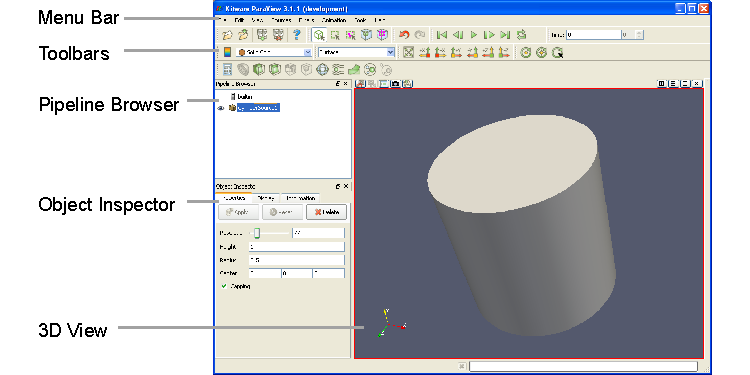
\includegraphics{images/UserInterface}
\end{inlinefig}

The ParaView GUI conforms to the platform on which it is running, but on
all platforms it behaves basically the same.  The layout shown here is the
default layout given when ParaView is first started.  The GUI comprises the
following components.

\begin{description}
\item[Menu Bar] \index{menu bar} As with just about any other program, the
  menu bar allows you to access the majority of features.
\item[Toolbars] \index{toolbars} The toolbars provide quick access to the
  most commonly used features within ParaView.
\item[Pipeline Browser] \index{pipeline browser} ParaView manages the
  reading and filtering of data with a pipeline.  The pipeline browser
  allows you to view the pipeline structure and select pipeline objects.
  Redesigned for ParaView 3, the pipeline browser provides a convenient
  list of pipeline objects with an indentation style that shows the
  pipeline structure.
\item[Object Inspector] \index{object inspector} The object inspector
  allows you to view and change the parameters of the current pipeline
  object.  There are three tabs in the object inspector.  The
  \keyterm{Properties} tab presents the configurable options for the object
  behavior.  The \keyterm{Display} tab presents options for how the object
  is represented in the view.  The \keyterm{Information} tab shows basic
  statistics on the data produced by the pipeline object.
\item[3D View] \index{3D View} The remainder of the GUI is used to present
  data so that you may view, interact with, and explore your data.  This
  area is initially populated with a 3D view that will provide a geometric
  representation of the data.
\end{description}

Note that the GUI layout is highly configurable, so that it is easy to
change the look of the window.  The toolbars can be moved around and even
hidden from view.  To toggle the use of a toolbar, use the \gui{View} \ra
\gui{Toolbars} submenu.  The pipeline browser and object inspector are both
\keyterm{dockable} windows.  This means that these components can be moved
around in the GUI, torn off as their own floating windows, or hidden
altogether.  These two windows are important to the operation of ParaView,
so if you hide them and then need them again, you can get them back with
the \gui{View} menu.


\section{Sources}

There are two ways to get data into ParaView: read data from a file or
generate data with a \keyterm{source} object.  All sources are located in
the \gui{Sources} menu.  Sources can be used to add annotation to a view,
but they are also very handy when exploring ParaView’s features.

\begin{exercise}{Creating a Source}
  \label{ex:CreatingASource}
  Let us start with a simple one.  Go to the \gui{Sources} menu and select
  \gui{Cylinder}.  Once you select the \gui{Cylinder} item you will notice
  that an item named \gui{Cylinder1} is added to and selected in the
  pipeline browser.  You will also notice that the object inspector is
  filled with the properties for the cylinder source.  Click the
  \gui{Apply} button \apply to accept the default parameters.

  Once you click \gui{Apply}, the cylinder object will be displayed in the
  3D view window on the right.  You can manipulate this 3D view by dragging
  the mouse over the 3D view.  Experiment with dragging different mouse
  buttons---left, middle, and right---to perform different rotate, pan, and
  zoom operations.  Also try using the buttons in conjunction with the
  shift and ctrl modifier keys.

  You will quickly notice that ParaView creates not a real cylinder but
  rather an approximation of a cylinder using polygonal \keyterm{facets}.
  The default parameters for the cylinder source provide a very coarse
  approximation of only six facets. (In fact, this object looks more like a
  prism than a cylinder.) If we want a better representation of a cylinder,
  we can create one by increasing the \gui{Resolution} parameter.

  \begin{inlinefig}
    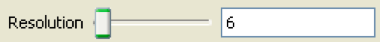
\includegraphics[width=2.5in]{images/ResolutionParameter}
  \end{inlinefig}

  Using either the slider or text edit, increase the resolution to 50 or
  more.  Notice that the \gui{Apply} button \apply has turned green (or
  blue on Mac) again.  This is because changes you make to the object
  inspector are not immediately enacted.  The highlighted button is a
  reminder that the parameters of one or more pipeline objects are ``out of
  sync'' with the data that you are viewing.  Hitting the \gui{Apply} button
  will accept these changes whereas hitting the \gui{Reset} button \reset
  will revert the options back to the last time they were applied.  Hit the
  \gui{Apply} button now.  The resolution is changed so that it is
  virtually indistinguishable from a true cylinder.
\end{exercise}

Now is a good time to note the undo~\icon{pqUndo32} and
redo~\icon{pqRedo32} buttons in the toolbar.  Visualizing your data is
often an exploratory process, and it is often helpful to revert back to a
previous state.  You can even undo back to the point before your data was
created and redo again.

\begin{exercise}{Undo and Redo}
  \label{ex:UndoAndRedo}
  Experiment with the undo~\icon{pqUndo32} and redo~\icon{pqRedo32}
  buttons.  If you have not done so, create and modify a pipeline object
  like what is done in Exercise~\ref{ex:CreatingASource}.  Watch how
  parameter changes can be reverted and restored.  Also notice how whole
  pipeline objects can be destroyed and recreated.

  There are also special undo camera~\icon{pqUndoCamera24} and redo
  camera~\icon{pqRedoCamera24} buttons.  These allow you to go back and
  forth between camera angles that you have made so that you no longer have
  to worry about errant mouse movements ruining that perfect view.  Move
  the camera around and then use these buttons to revert and restore the
  camera angle.
\end{exercise}

There are also many options for selecting how objects are rendered.  You
will notice over the 3D view a \icon{pqOptions16} button for changing the
rendering options.  Clicking this brings up a dialog box that allows you to
change things like the background color, the lighting, and annotation.

\begin{inlinefig}
  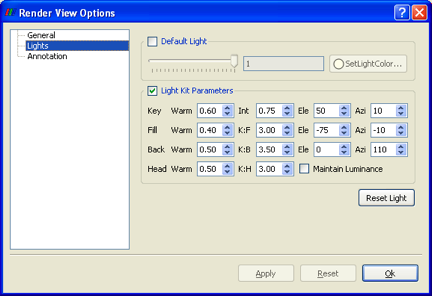
\includegraphics[width=3in]{images/RenderViewOptions}
\end{inlinefig}

Another location for rendering options is the \gui{Display} tab in the
object inspector.  This tab provides the rendering options that apply
specifically for the selected object.  It includes the visibility,
coloring, and representation.  Be aware that some of the view options and
object display options are repeated elsewhere in the ParaView GUI for
convenience.

\begin{inlinefig}
  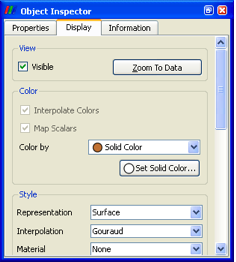
\includegraphics[width=1.6in]{images/DisplayTab}
\end{inlinefig}

\begin{exercise}{Modifying Rendering Parameters}
  \label{ex:ModifyingRenderingParameters}
  Click the \icon{pqOptions16} button above the 3D view to bring up the
  \gui{Render View Options} dialog box.  Explore the different panels of
  options.  Try modifying how the view looks in the following ways.
  (Remember that you will have to hit \gui{Apply} or \gui{OK} before the
  changes take effect.)

  \begin{itemize}
  \item Change the background color.  (Notice that you can reset it to the
    default.)
  \item Turn the Orientation Axis (the axis in the lower left corner of the
    view) off and on.
  \item Move the Orientation Axis in the view.  (Hint: Make the axis
    interactive and then click and drag in the 3D view.)
  \end{itemize}

  Now change the drawing parameters of the cylinder.  (If you do not have a
  cylinder or another pipeline object, create one as described in
  Exercise~\ref{ex:CreatingASource}.)  Make sure the cylinder is selected
  in the pipeline browser.  In the object inspector, select the
  \gui{Display} tab.

  \begin{itemize}
  \item Set the (solid) color of the cylinder.  (Note: You can also set the
    color with the \icon{pqEditColor24} toolbar button.)
  \item Make the cylinder shiny.  (Hint: Make the \gui{Specular Intensity}
    1.0.)
  \item Make the cylinder transparent.  (Hint: Lower the \gui{Opacity}.)
  \item Show 3D axes with tic marks giving spatial position (\gui{Show cube
    axes}).
  \end{itemize}

  We are done with the cylinder source now.  We can delete the pipeline
  object by selecting the \gui{Properties} tab and hitting delete \delete
  in the object inspector.
\end{exercise}


\section{Loading Data}

Now that we have had some practice using the ParaView GUI, let us load in
some real data.  As you would expect, the \gui{Open} command is the first
one off of the \gui{File} menu, and there is also toolbar
button~\icon{pqOpen32} for opening a file.  ParaView supports many file
types, and the list grows as more types get added.  The following is a list
of currently available readers.

\begin{multicols}{2}
  \begin{itemize}
  \item ParaView Data (.pvd)
  \item VTK (.vtp, .vtu, .vti, .vts, .vtr)
  \item VTK Multi Block (.vtm, .vtmb, .vtmg, .vthd, .vthb)
  \item Partitioned VTK (.pvtu, .pvti, .pvts, .pvtr)
  \item VTK Legacy (.vtk)
  \item Exodus
  \item XDMF (.xmf, .xdmf)
  \item LS-DYNA
  \item SpyPlot CTH
  \item EnSight (.case, .sos)
  \item netCDF (.ncdf, .nc)
  \item BYU (.g)
  \item Protein Data Bank (.pdb)
  \item XMol Molecule
  \item PLOT3D
  \item Digital Elevation Map (.dem)
  \item VRML (.wrl)
  \item PLY Polygonal File Format
  \item Stereo Lithography (.stl)
  \item Gaussian Cube File (.cube)
  \item POP Ocean Files
  \item AVS UCD (.inp)
  \item Meta Image (.mhd, .mha)
  \item Facet Polygonal Data
  \item Phasta Files (.pht)
  \item SESAME Tables
  \item MFIX (.RES)
  \item Fluent Case Files (.cas)
  \item OpenFOAM Files (.foam)
  \item Cosmology Files (.cosmo)
  \item PNG Image Files
  \item TIFF Image Files
  \item Raw Image Files
  \item Comma Separated Values (.csv)
  \end{itemize}
\end{multicols}

ParaView’s modular design allows for easy integration of new VTK readers
into ParaView.  Thus, check back often for new file formats.  If you are
looking for a file reader that does not seem to be included with ParaView,
check in with the ParaView mailing list
(\href{mailto:paraview@paraview.org}{paraview@paraview.org}).  There are
many file readers included with VTK but not exposed within ParaView that
could easily be added.  There are also many readers created that can plug
into the VTK framework but have not been committed back to VTK; someone may
have a reader readily available that you can use.

\begin{exercise}{Opening a File}
  \label{ex:OpeningAFile}
  Let us open our first file now.  Click the \gui{Open} toolbar (or menu
  item)~\icon{pqOpen32} and open the file \gui{disk\_out\_ref.ex2}.  Note
  that opening a file is a two step process, so that you do not see any
  data yet.  Instead, you see that the object inspector is populated with
  several options about how we want to read the data.

  \begin{inlinefig}
    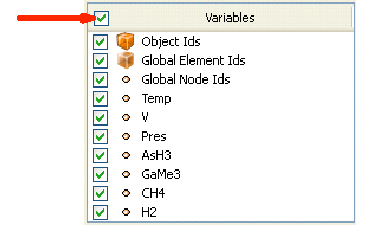
\includegraphics{images/Variables_disk_out_ref}
  \end{inlinefig}

  Click the checkbox in the header of the variable list to turn on the
  loading of all the variables.  This is a small data set, so we do not
  have to worry about loading too much into memory.  Once all of the
  variables are selected, click \apply to load all of the data.  When the
  data is loaded you will see that the geometry looks like a cylinder with
  a hollowed out portion in one end.  This data is the output of a
  simulation for the flow of air around a heated and spinning disk.  The
  mesh you are seeing is the air around the disk (with the cylinder shape
  being the boundary of the simulation.  The hollow area in the middle is
  where the heated disk would be were it meshed for the simulation.
\end{exercise}

Before we continue on to filtering the data, let us take a quick look at
some of the ways to represent the data.  The most common parameters for
representing data are located in a pair of toolbars.

\begin{inlinefig}
  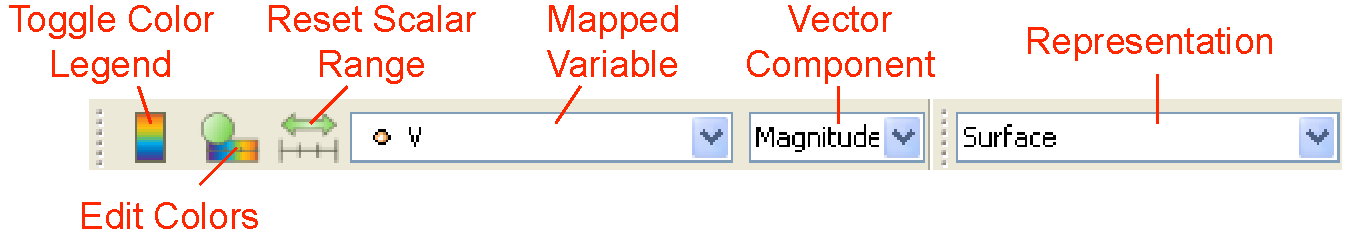
\includegraphics[width=\linewidth]{images/DataRepresentationToolbars}
\end{inlinefig}

\begin{exercise}{Representation and Field Coloring}
  \label{ex:RepresentationAndFieldColoring}
  Play with the data representation a bit.  Make sure
  \gui{disk\_out\_ref.ex2} is selected in the pipeline browser.  (If you do
  not have the data loaded, repeat Exercise~\ref{ex:OpeningAFile}.)  Use
  the variable chooser to color the surface by the \gui{Pres} variable.
  Then turn the color legend on to see the actual pressure values.  To see
  the structure of the mesh, change the representation to \gui{Surface With
    Edges}.  You can view both the cell structure and the interior of the
  mesh with the \gui{Wireframe} representation.

  \begin{inlinefig}
    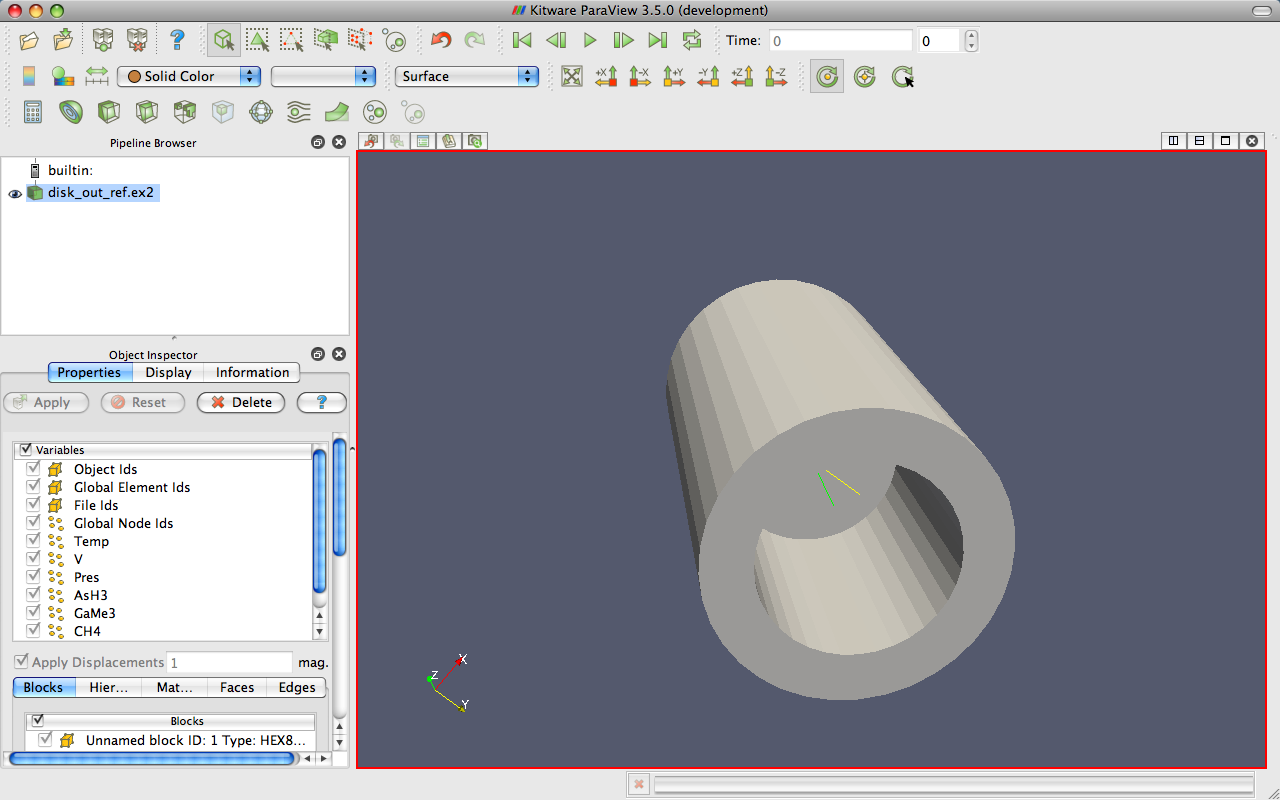
\includegraphics[width=2.25in]{images/DataRepresentation1}
    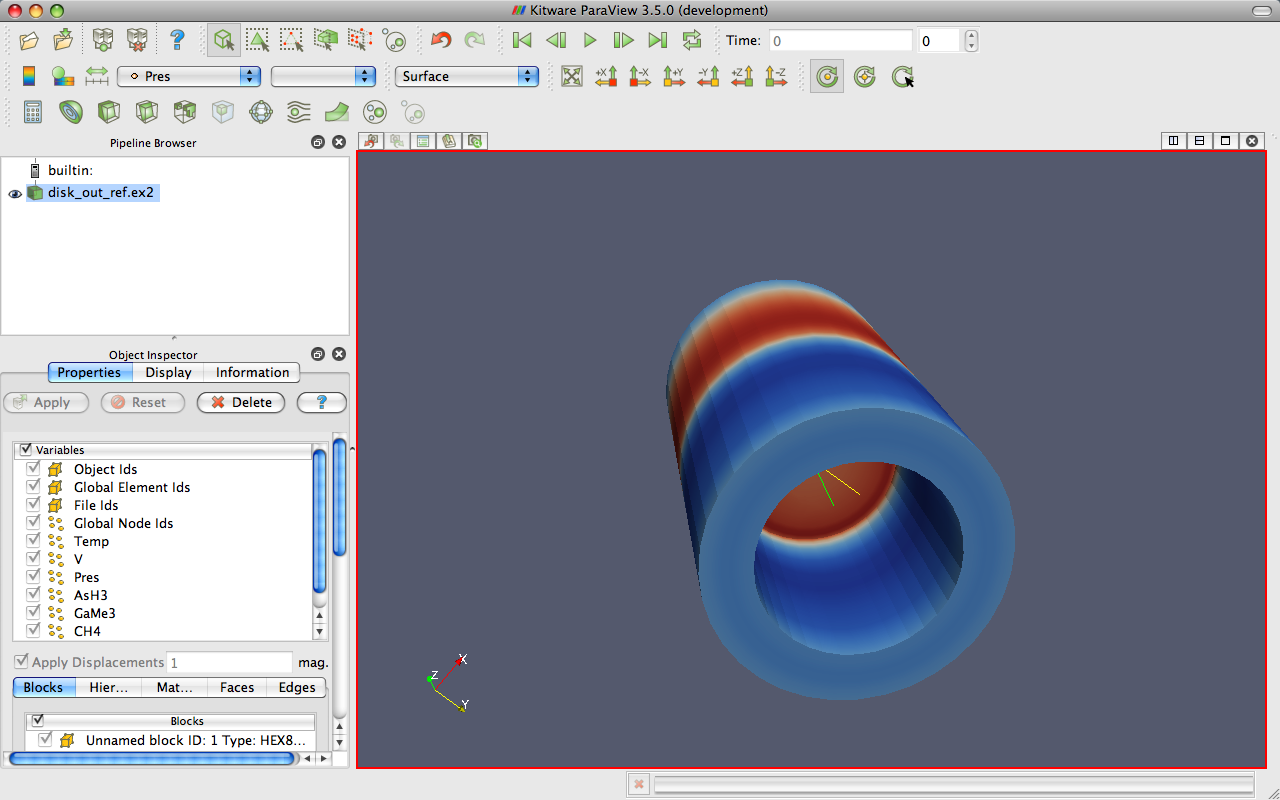
\includegraphics[width=2.25in]{images/DataRepresentation2} \\
    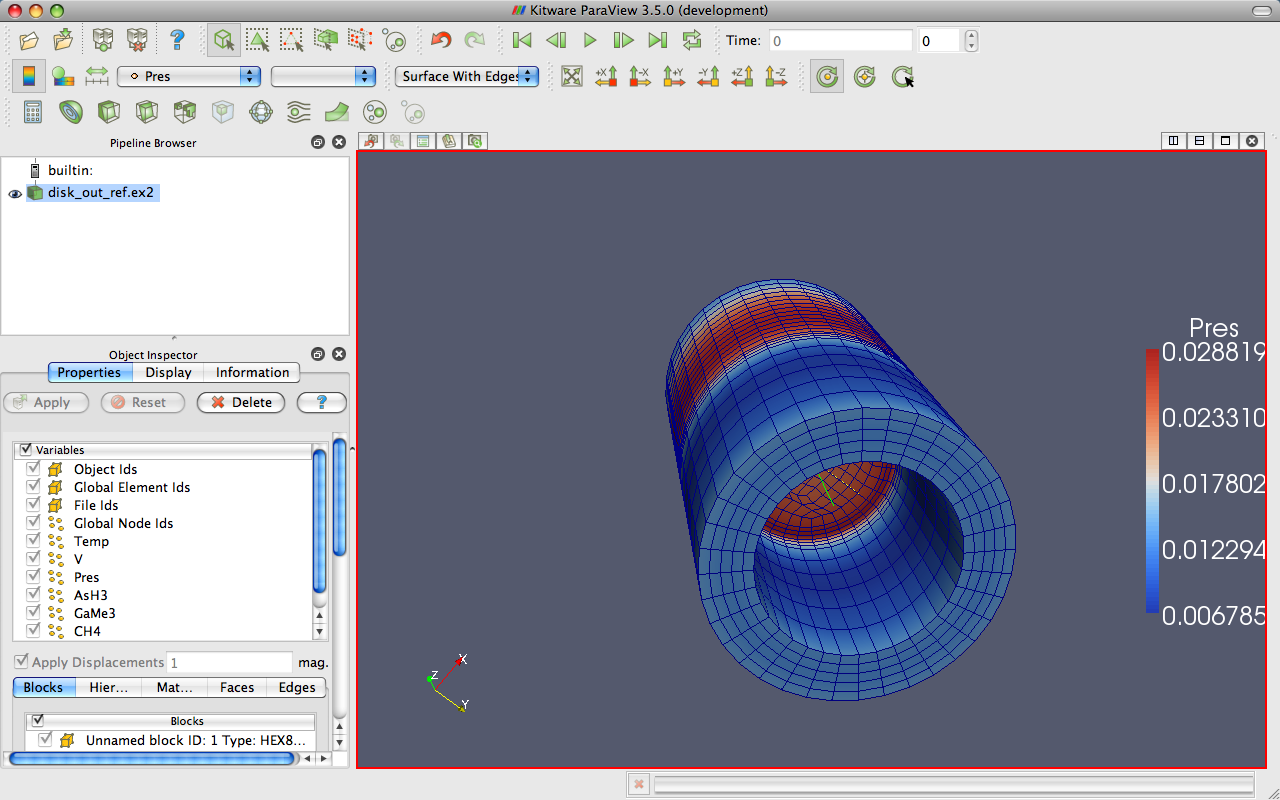
\includegraphics[width=2.25in]{images/DataRepresentation3}
    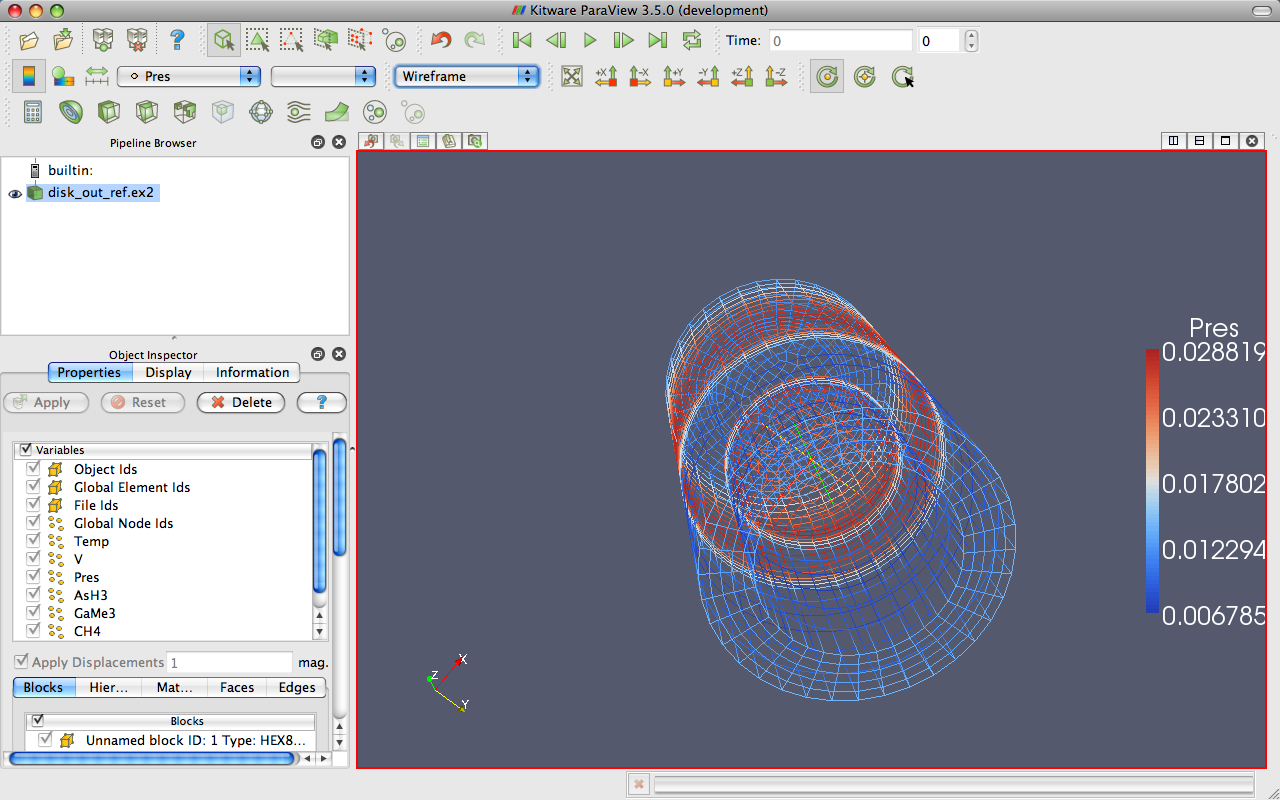
\includegraphics[width=2.25in]{images/DataRepresentation4}
  \end{inlinefig}
\end{exercise}


\section{Filters}

We have now successfully read in some data and gleaned some information
about it.  We can see the basic structure of the mesh and map some data
onto the surface of the mesh.  However, as we will soon see, there are many
interesting features about this data that we cannot determine by simply
looking at the surface of this data.  There are many variables associated
with the mesh of different types (scalars and vectors).  And remember that
the mesh is a solid model.  Most of the interesting information is on the
inside.

We can discover much more about our data by applying \keyterm{filters}.
Filters are functional units that process the data to generate, extract, or
derive features from the data.  Filters are attached to readers, sources,
or other filters to modify its data in some way.  These filter connections
form a \keyterm{visualization pipeline}.  There are a great many filters
available in ParaView.  Here are the most common, which are all available
by clicking on the respective icon in the filters toolbar.

\begin{description}
\item[\calculator Calculator] \index{calculator} Evaluates a user-defined
  expression on a per-point or per-cell basis.
\item[\contour Contour] \index{contour} Extracts the points, curves, or
  surfaces where a scalar field is equal to a user-defined value.  This
  surface is often also called an \keyterm{isosurface}.
\item[\clip Clip] \index{clip} Intersects the geometry with a half space.
  The effect is to remove all the geometry on one side of a user-defined
  plane.
\item[\slice Slice] \index{slice} \index{cut|see{slice}} Intersects the
  geometry with a plane.  The effect is similar to clipping except that all
  that remains is the geometry where the plane is located.
\item[\threshold Threshold] \index{threshold} Extracts cells that lie
  within a specified range of a scalar field.
\item[\extractSubset Extract Subset] \index{extract subset} Extracts a
  subset of a grid by defining either a volume of interest or a sampling
  rate.
\item[\glyph Glyph] Places a \keyterm{glyph}, a simple shape, on each point
  in a mesh.  The glyphs may be oriented by a vector and scaled by a vector
  or scalar.
\item[\streamTracer Stream Tracer] \index{stream tracer} Seeds a vector
  field with points and then traces those seed points through the (steady
  state) vector field.
\item[\warp Warp (vector)] \index{warp!vector} Displaces each point in a
  mesh by a given vector field.
\item[\group Group Datasets] \index{group datasets} Combines the output of
  several pipeline objects into a single multi block data set.
\item[\extractGroup Extract Group] \index{extract group} Extract one or
  more items from a multi block data set.
\end{description}

\parpic[r]{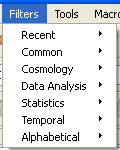
\includegraphics[width=2in]{images/FiltersMenu}}

These eleven filters are a small sampling of what is available in ParaView.
In the \gui{Filters} menu are a great many more filters that you can use to
process your data.  ParaView currently exposes over eighty filters, so to
make them easier to find the \gui{Filters} menu is organized into submenus.
These submenus are organized as follows.

\begin{description}
\item[Recent] The list of most recently used filters sorted with the most
  recently used filters on top.
\item[Common] The most common filters.  This is the same list of filters
  available in the filters toolbar and listed previously.
\item[Data Analysis] The filters designed to retrieve quantitative values
  from the data.  These filters compute data on the mesh, extract elements
  from the mesh, or plot data.
\item[Temporal] Filters that analyze or modify data that changes over time.
  All filters can work on data that changes over time because they are
  executed on each time snapshot.  However, filters in this category will
  introspect the available time extents and examine how data changes over
  time.
\item[Alphabetical] An alphabetical listing of all the filters available.
  If you are not sure where to find a particular filter, this list is
  guaranteed to have it.  There are also many filters that are not listed
  anywhere but in this list.
\end{description}

You have probably noticed that some of the filters are grayed out.  Many
filters only work on a specific types of data and therefore cannot always
be used.  ParaView disables these filters from the menu and toolbars to
indicate (and enforce) that you cannot use these filters.

Throughout this tutorial we will explore many filters.  However, we cannot
explore all the filters in this forum.  Consult \emph{The ParaView Guide}
for more information on each filter.

\begin{exercise}{Apply a Filter}
  \label{ex:ApplyAFilter}
  Let us apply our first filter.  If you do not have the disk\_out\_ref.ex2
  data loaded, do so know (Exercise~\ref{ex:OpeningAFile}).  Make sure that
  \gui{disk\_out\_ref.ex2} is selected in the pipeline browser and then
  select the contour filter~\contour from the filter toolbar or
  \gui{Filters} menu.  Notice that a new item is added to the pipeline
  filter underneath the reader and the object inspector updates to the
  parameters of the new filter.  As with reading a file, applying a filter
  is a two step process.  After creating the filter you get a chance to
  modify the parameters (which you will almost always do) before applying
  the filter.

  \begin{inlinefig}
    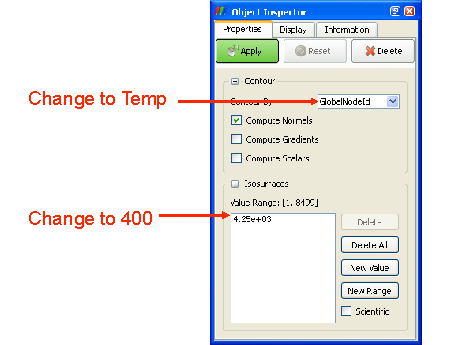
\includegraphics{images/ContourOptions}
  \end{inlinefig}

  We will use the contour filter to create an isosurface where the
  temperature is equal to 400 K.  First, change the \gui{Contour By}
  parameter to the \gui{Temp} variable.  Then, change the isosurface value
  to \gui{400}.  Finally, hit \apply.  You will see the isosurface appear
  inside of the volume.  If \gui{disk\_out\_ref.ex2} was still colored by
  pressure from Exercise~\ref{ex:RepresentationAndFieldColoring}, then the
  surface is colored by pressure to match.

  \begin{inlinefig}
    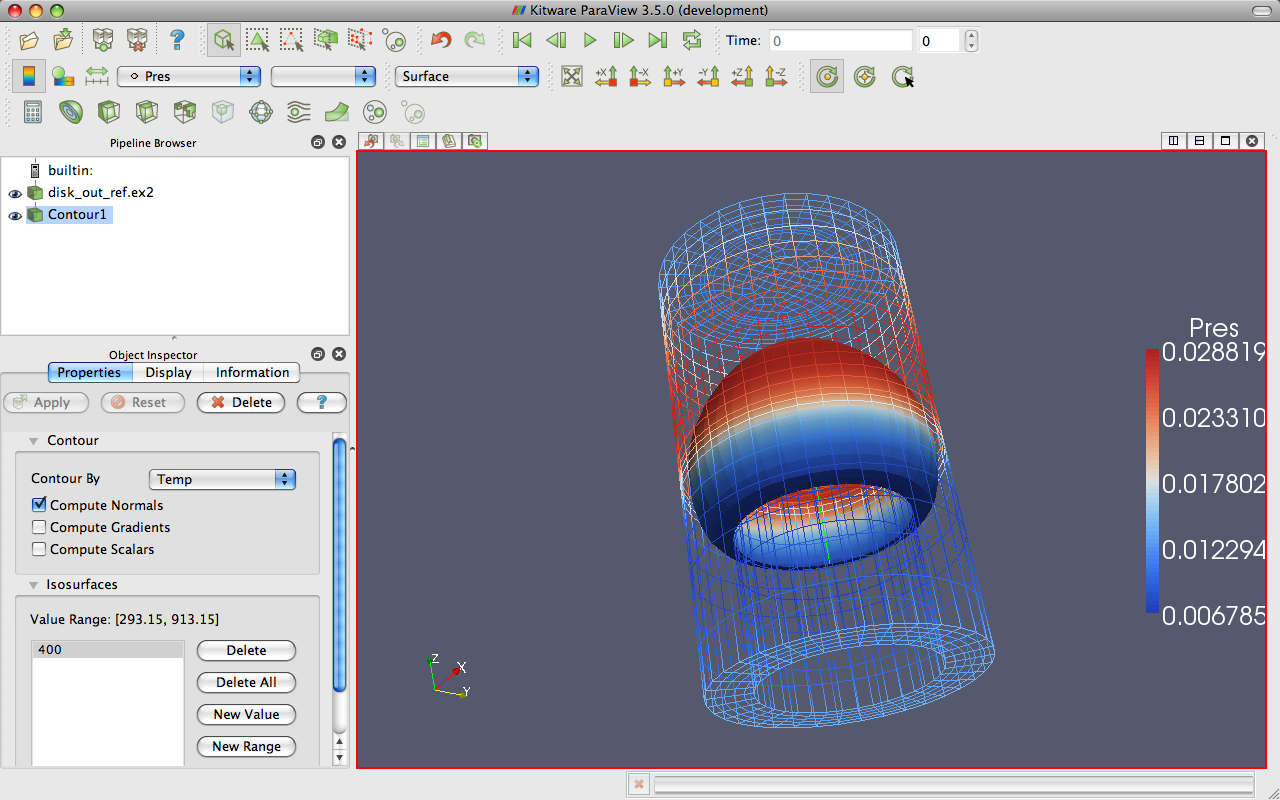
\includegraphics[width=3in]{images/ContourResults}
  \end{inlinefig}
\end{exercise}

In the preceding exercise, we applied a filter that processed the data and
gave us the results we needed.  For most common operations, a single filter
operation is sufficient to get the information we need.  However, filters
are of the same class as readers.  That is, the general operations we apply
to readers can also be applied to filters.  Thus, you can apply one filter
to the data that is generated by another filter.  These readers and filters
connected together form what we call a \keyterm{visualization pipeline}.
The ability to form visualization pipelines provides a powerful mechanism
for customizing the visualization to your needs.

Let us play with some more filters.  Rather than show the mesh surface in
wireframe, which often interferes with the view of what is inside it, we
will replace it with a cutaway of the surface.  We need to filters to
perform this task.  The first filter will extract the surface, and the
second filter will cut some away.

\begin{exercise}{Creating a Visualization Pipeline}
  \label{ex:CreatingAVisualizationPipeline}
  The images and some of the discussion in this exercise assume you are
  starting with the state right after finishing
  Exercise~\ref{ex:ApplyAFilter}.  If you have had to restart ParaView
  since or your state does not match up well enough, it is sufficient to
  simply have disk\_out\_ref.ex2 loaded.

  Start by adding a filter that will extract the surfaces.  We do that with
  the following steps.

  \begin{enumerate}
  \item Select \gui{disk\_out\_ref.ex2} in the pipeline browser.
  \item From the menu bar, select \gui{Filters} \ra \gui{Alphabetical} \ra
    \gui{Extract Surface}. \index{extract surface}
  \item Hit the \apply button.
    \savecounter
  \end{enumerate}

  \begin{inlinefig}
    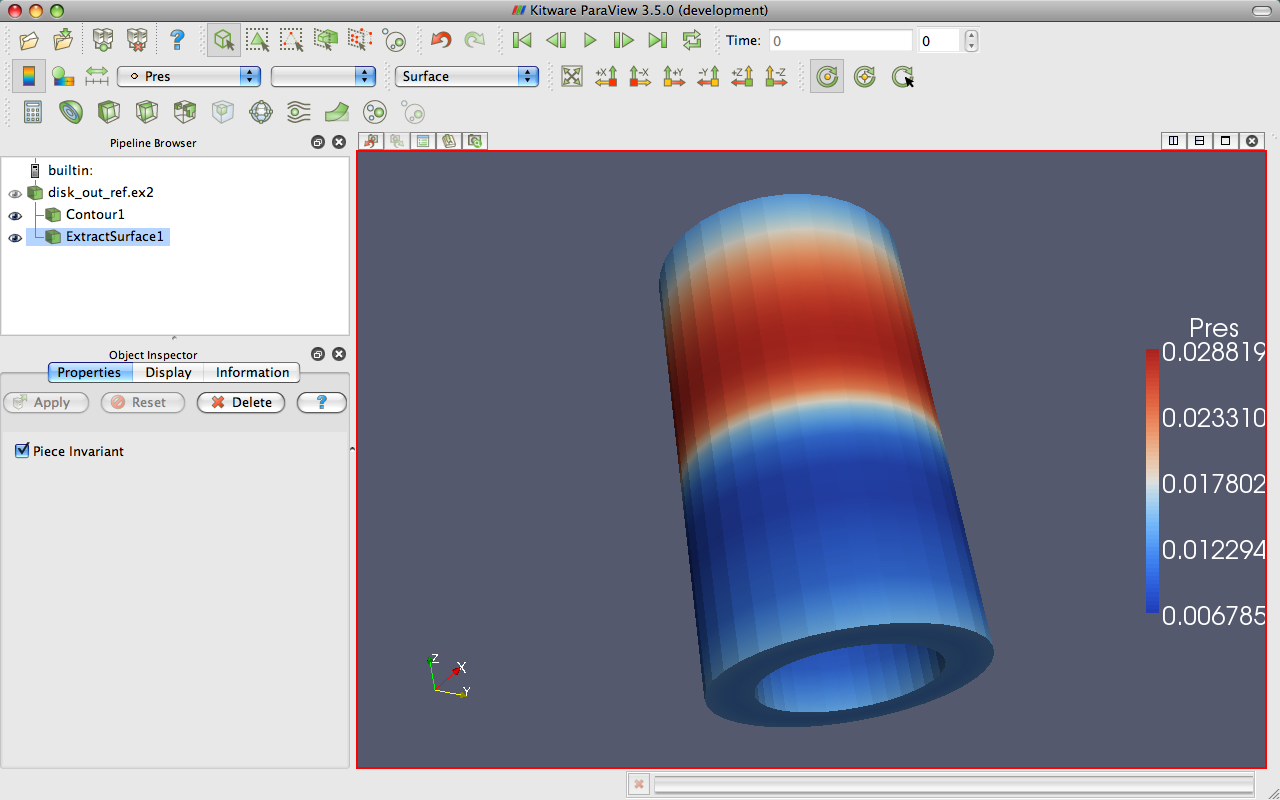
\includegraphics[width=3in]{images/CutSurface1}
  \end{inlinefig}

  When you apply the \gui{Extract Surface} filter, you will once again see
  the surface of the mesh.  Although it looks like the original mesh, it is
  different in that this data is hollow whereas the original data was solid
  throughout.

  If you were showing the results of the contour filter, you cannot see the
  contour anymore, but do not worry.  It is still in there hidden by the
  surface.  If you are showing the contour but you did not see any effect
  after applying the filter, you may have forgotten step one and applied
  the filter to the wrong object.  If the \gui{ExtractSurface1} object is
  not connected directly to the \gui{disk\_out\_ref.ex2}, then this is what
  went wrong.  If so, you can delete the filter and try again.

  Now we will cut away the external surface to expose the internal
  structure and isosurface underneath (if you have one).

  \begin{enumerate}
    \restorecounter
  \item Verify that \gui{ExtractSurface1} is selected in the pipeline
    browser.
  \item Create a clip filter \clip from the toolbar or \gui{Filters} menu.
  \item Uncheck the \gui{Show Plane} checkbox
    \includeinlinegraphics{images/ShowPlaneCheckbox} in the object inspector.
  \item Click the \apply button.
  \end{enumerate}

  \begin{inlinefig}
    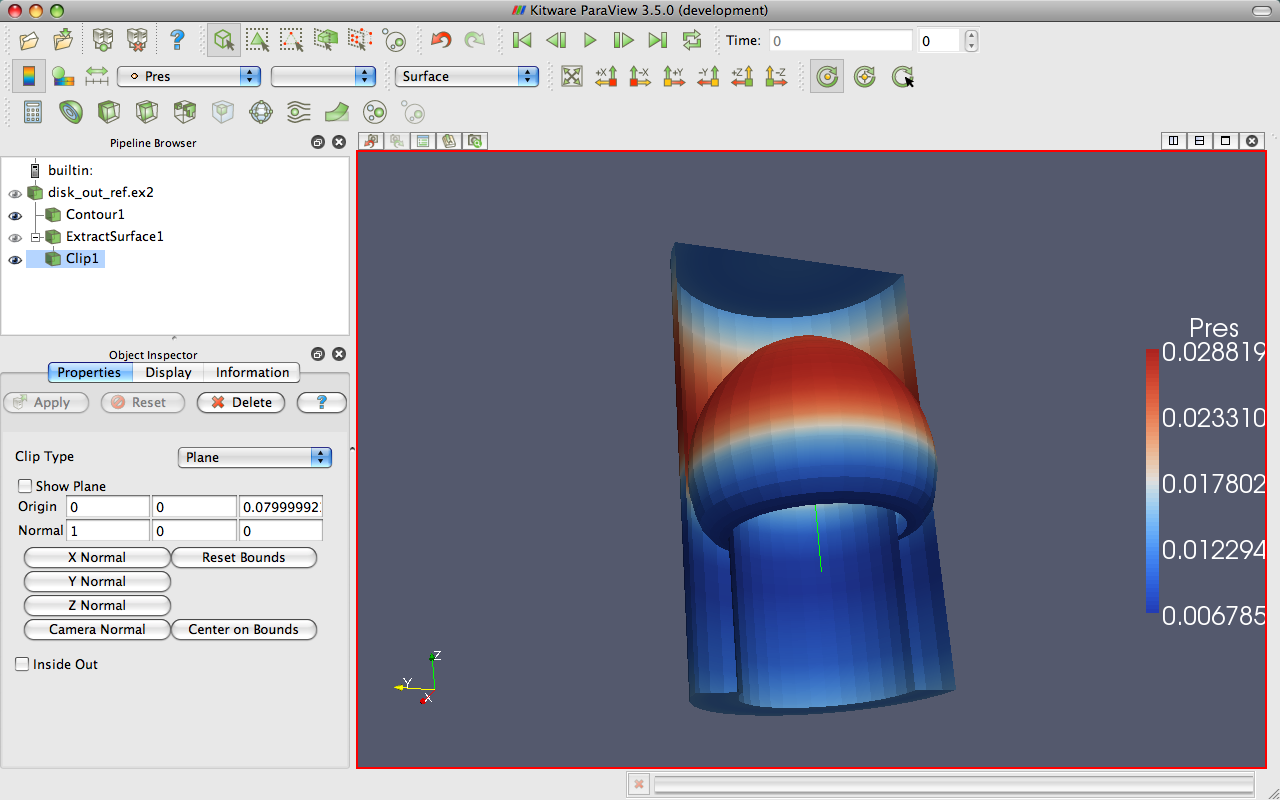
\includegraphics[width=3in]{images/CutSurface2}
  \end{inlinefig}

  If you have a contour, you should now see the isosurface contour within a
  cutaway of the mesh surface.  You will probably have to rotate the mesh
  to see the contour clearly.
\end{exercise}

\begin{inlinefig}
  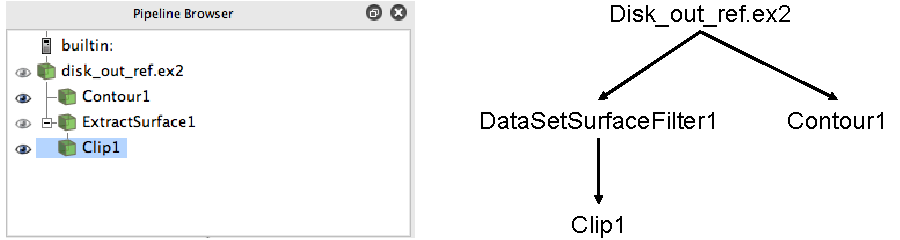
\includegraphics[width=\linewidth]{images/PipelineBrowserStructure}
\end{inlinefig}

Now that we have added several filters to our pipeline, let us take a look
at the layout of these filters in the pipeline browser.  The pipeline
browser provides a convenient list of pipeline objects that we have created
make it easy to select pipeline objects and change their
\keyterm{visibility} by clicking on the eyeball icons~\eyeball next to
them.  But also notice the indentation of the entries in the list and the
connecting lines toward the right.  These features reveal the
\keyterm{connectivity} of the pipeline.  It shows the same information as
the traditional graph layout on the right, but in a much more compact
space.  The trouble with the traditional layout of pipeline objects is that
it takes a lot of space, and even moderately sized pipelines require a
significant portion of the GUI to see fully.  The pipeline browser,
however, is complete and compact.


\section{Multiview}
\label{sec:Multiview}

Occasionally in the pursuit of science we can narrow our focus down to one
variable.  However, most interesting physical phenomena rely on not one but
many variables interacting in certain ways.  It can be very challenging to
present many variables in the same view.  To help you explore complicated
visualization data, ParaView contains the ability to present multiple views
of data and correlate them together.

So far in our visualization we are looking at two variables: We are
coloring with pressure and have extracted an isosurface with temperature.
Although we are starting to get the feel for the layout of these variables,
it is still difficult to make correlations between them.  To make this
correlation easier, we can use multiple views.  Each view can show an
independent aspect of the data and together they may show a more complete
understanding.

On top of each view is a small toolbar, and the buttons controlling the
creating and deletion of views are located on the right side of this tool
bar.  There are four buttons in all.  You can create a new view by
splitting an existing view horizontally or vertically with the \splitViewH
and \splitViewV buttons, respectively.  The \deleteView button deletes a
view, whose space is consumed by an adjacent view.  The \maximizeView
temporarily fills view space with the selected view until \restoreView is
pressed.  Press the \splitViewH button now.

\begin{inlinefig}
  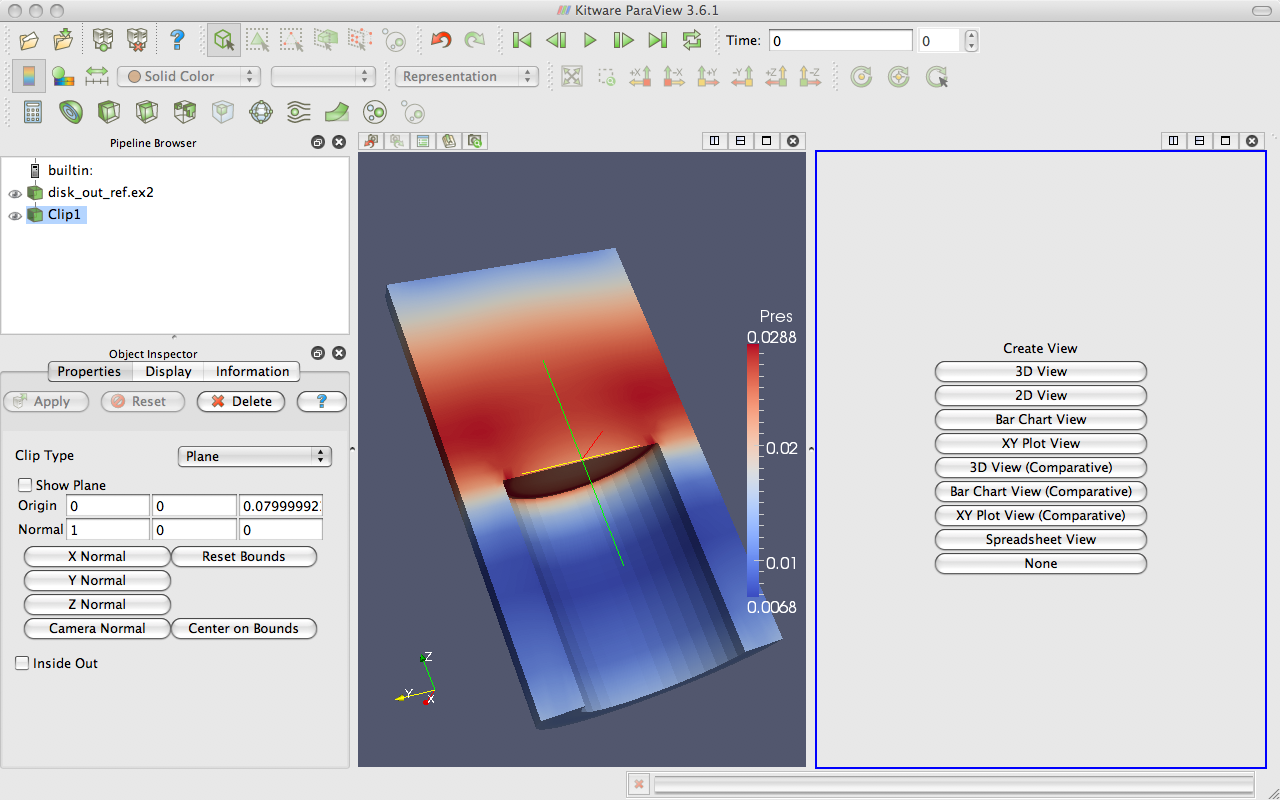
\includegraphics[width=3in]{images/SplitView1}
\end{inlinefig}

The current view is split in half and the right side is blank, ready to be
filled with a new visualization.  Notice that the view in the right has a
red border around it.  This means that it is the \keyterm{active view}.
Widgets that give information about and controls for a single view,
including the pipeline browser and object inspector, follow the active
view.  In this new view we will visualize the temperature of the mesh.

\begin{enumerate}
\item Make sure the red border is still around the new, blank view (to the
  right).  You can make any view the active view by simply clicking on it.
\item Turn on the visibility of the original data by clicking the
  eyeball~\eyeballg next to \gui{disk\_out\_ref.ex2} in the pipeline
  browser.
\item Color the surface by temperature by selecting
  \gui{disk\_out\_ref.ex2} in the pipeline browser and changing the
  variable chooser (in the toolbar) from \gui{Solid Color} to \gui{Temp}
  (you may want to turn on the color bar at this point as well).
  \savecounter
\end{enumerate}
We can see the color on the outside of the mesh, but it is not very
interesting and the boundaries.  We need to clip away the mesh to see the
temperature on the inside.
\begin{enumerate}
  \restorecounter
\item Add the Clip filter~\clip to \gui{disk\_out\_ref.ex2}.
\item Uncheck the Show Plane checkbox
  \includeinlinegraphics{images/ShowPlaneCheckbox} in the object inspector.
\item Click the \apply button.
\end{enumerate}

\begin{inlinefig}
  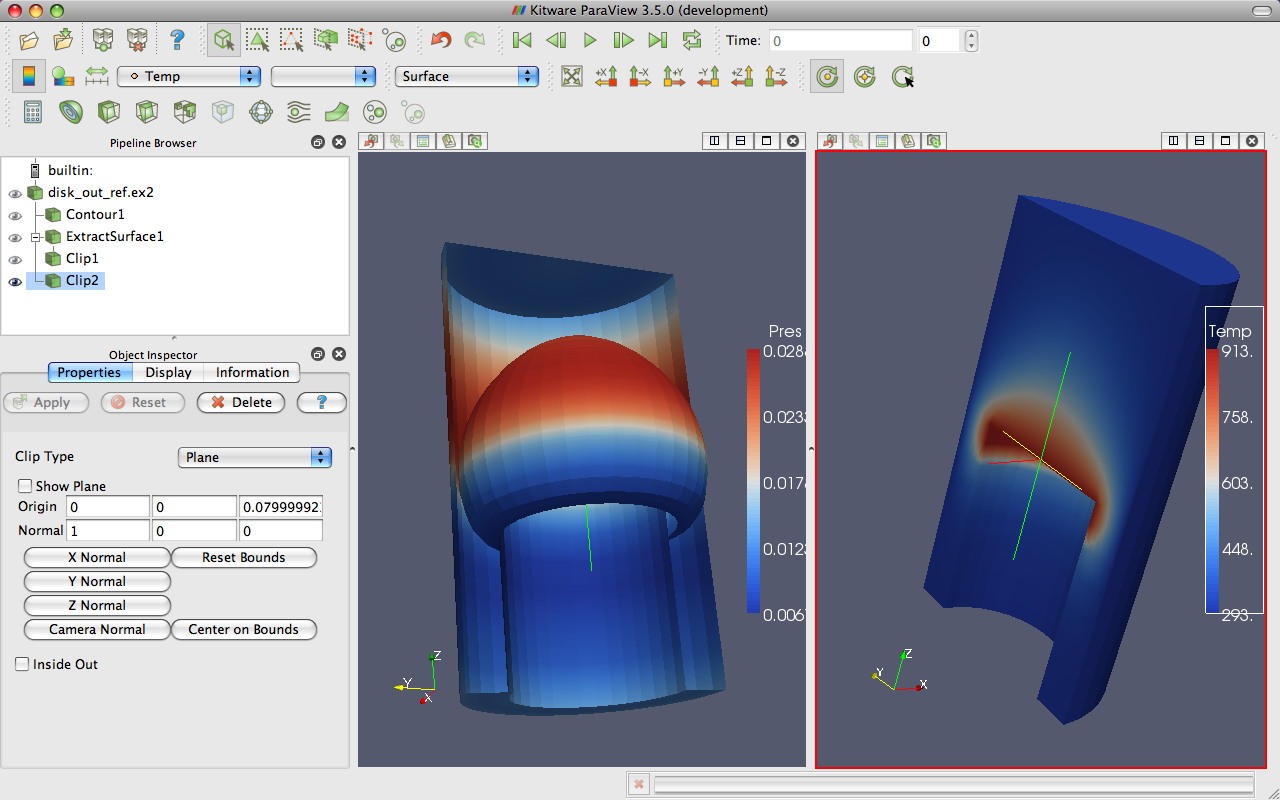
\includegraphics[width=3in]{images/SplitView2}
\end{inlinefig}

We now have two views: one showing information about pressure and the other
information about temperature.  We would like to compare these, but it is
difficult to do because the orientations are different.  How are we to know
how a location in one correlates to a location in the other.  We can solve
this problem by adding a \keyterm{camera link} so that the two views will
always be drawn from the same viewpoint.  Linking cameras is easy.  First
right click on one of the views and select \gui{Link Camera...} from the
pop up menu. (If you are on a Mac with no right mouse button, you can
perform the same operation with the menu option \gui{Tools} \ra \gui{Add
  Camera Link...})  Now click in a second view.  \emph{Viola}!  The two
cameras are linked; each will follow the other.

\begin{inlinefig}
  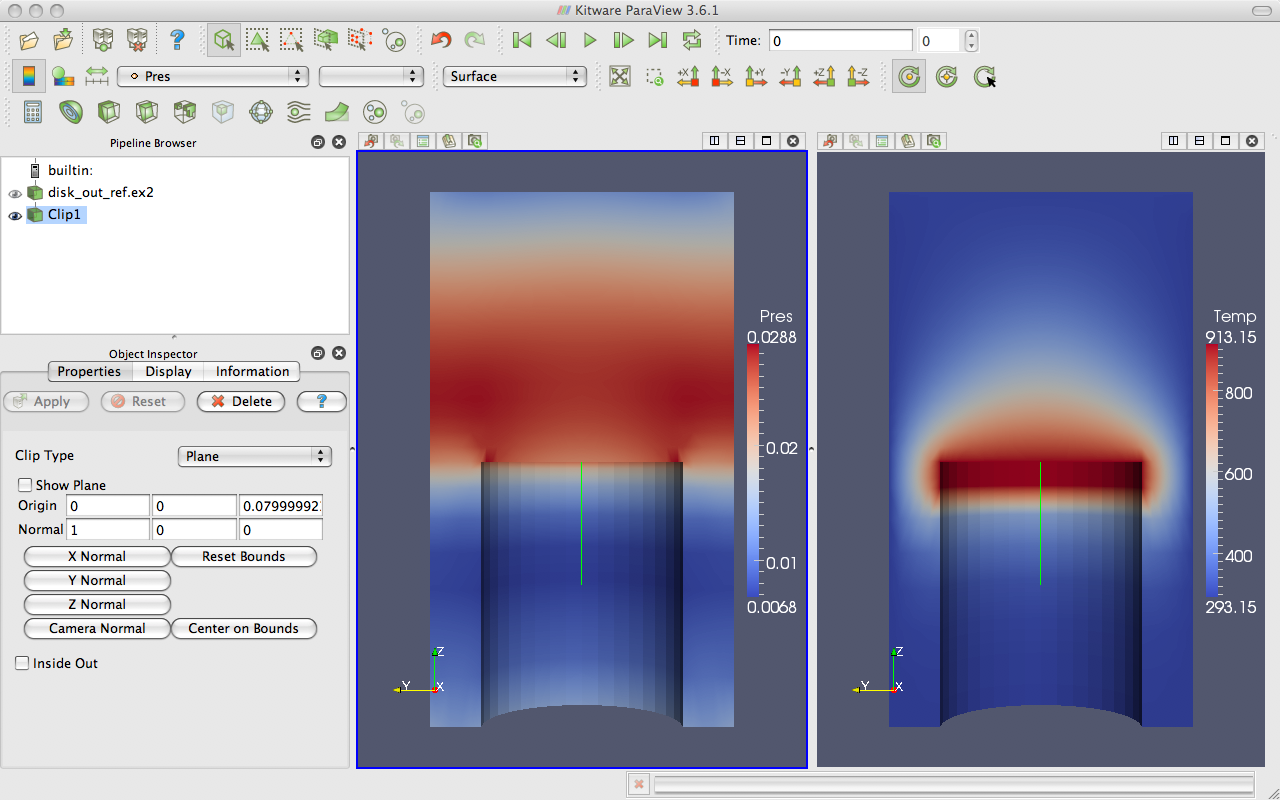
\includegraphics[width=3in]{images/CameraLink}
\end{inlinefig}

With the cameras linked, we can make some comparisons between the two
views.  Click the~\xPlus button to get a straight-on view of the cross section.
Notice that the temperature is highest at the interface with the heated
disk.  That alone is not surprising.  We expect the air temperature to be
greatest near the heat source and drop off away from it.  But notice that
at the same position the pressure is not maximal.  The air pressure is
maximal at a position above the disk.  Based on this information we can
draw some interesting hypotheses about the physical phenomenon.  We can
expect that there are two forces contributing to air pressure.  The first
force is that of gravity causing the upper air to press down on the lower
air.  The second force is that of the heated air becoming less dense and
therefore rising.  We can see based on the maximal pressure where these two
forces are equal.  Such an observation cannot be drawn without looking at
both the temperature and pressure in this way.

Multiview in ParaView is of course not limited to simply two windows.  Note
that each of the views has its own set of multiview buttons.  You can
create more views by using the split view buttons \splitViewH \splitViewV
to arbitrarily divide up the working space.  And you can delete views
\deleteView at any time.

\begin{inlinefig}
  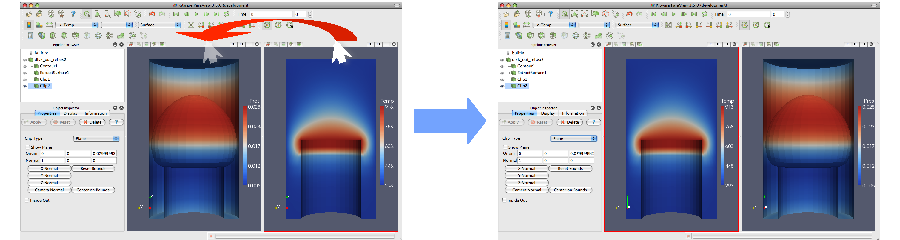
\includegraphics[width=\linewidth]{images/SwapViews}
\end{inlinefig}

The location of each view is also not fixed.  You are also able to swap two
views by clicking on one of the view toolbars (somewhere outside of where
the buttons are), holding down the mouse button, and dragging onto one of
the other view toolbars.  This will immediately swap the two views.

\begin{inlinefig}
  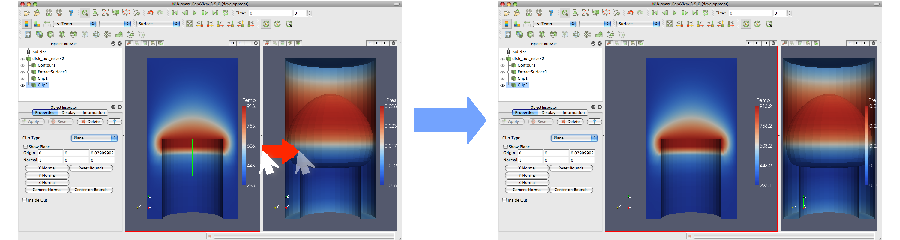
\includegraphics[width=\linewidth]{images/ResizeViews}
\end{inlinefig}

You can also change the size of the views by clicking on the space in
between views, holding down the mouse button, and dragging in the direction
of either one of the views.  The divider will follow the mouse and adjust
the size of the views as it moves.


\section{Further Exploration}

Let us see what else we can learn about this simulation.  The simulation
has also outputted a velocity field describing the movement of the air over
the heated rotating disk.  We will use ParaView to determine the currents
in the air.

Start with a fresh view so that we can preserve the previous views we have
already created.  Split one of the views vertically~\splitViewV, and then
maximize~\maximizeView the new view so that we can focus on it.  Make the
original data set visible by clicking the eyeball~\eyeballg next to
\gui{disk\_out\_ref.ex2} in the pipeline browser.  Visualize the air
currents by performing the following.

\begin{enumerate}
\item Select \gui{disk\_out\_ref.ex2} in the pipeline browser.
\item Add the stream tracer filter \streamTracer to
  \gui{disk\_out\_ref.ex2}.
\item Click the \apply button to accept the default parameters.
  \savecounter
\end{enumerate}

The surface of the mesh is replaced with some swirling lines.  The new
geometry is off-center from the previous geometry.  We can quickly center
the view on the new geometry with the \keyterm{reset camera}~\resetCamera
command.  This command centers and fits the visible geometry within the
current view and also resets the center of rotation to the middle of the
visible geometry.

The lines are difficult to distinguish because there are many close
together and they have no shading.  Lines are a 1D structure and shading
requires a 2D surface.  We can create a 2D surface around our stream traces
with the tube filter.

\begin{enumerate}
  \restorecounter
\item From the menu bar, select \gui{Filters} \ra \gui{Alphabetical} \ra
  \gui{Tube}\index{tube}.\footnote{In ParaView 3.6 the name of the tube
    filter was changed to \gui{Generate Tubes}.  In future versions, the
    name will change back to \gui{Tube} to make it easier to find in
    alphabetical filter lists.}
\item Hit the \apply button.
\end{enumerate}

\begin{inlinefig}
  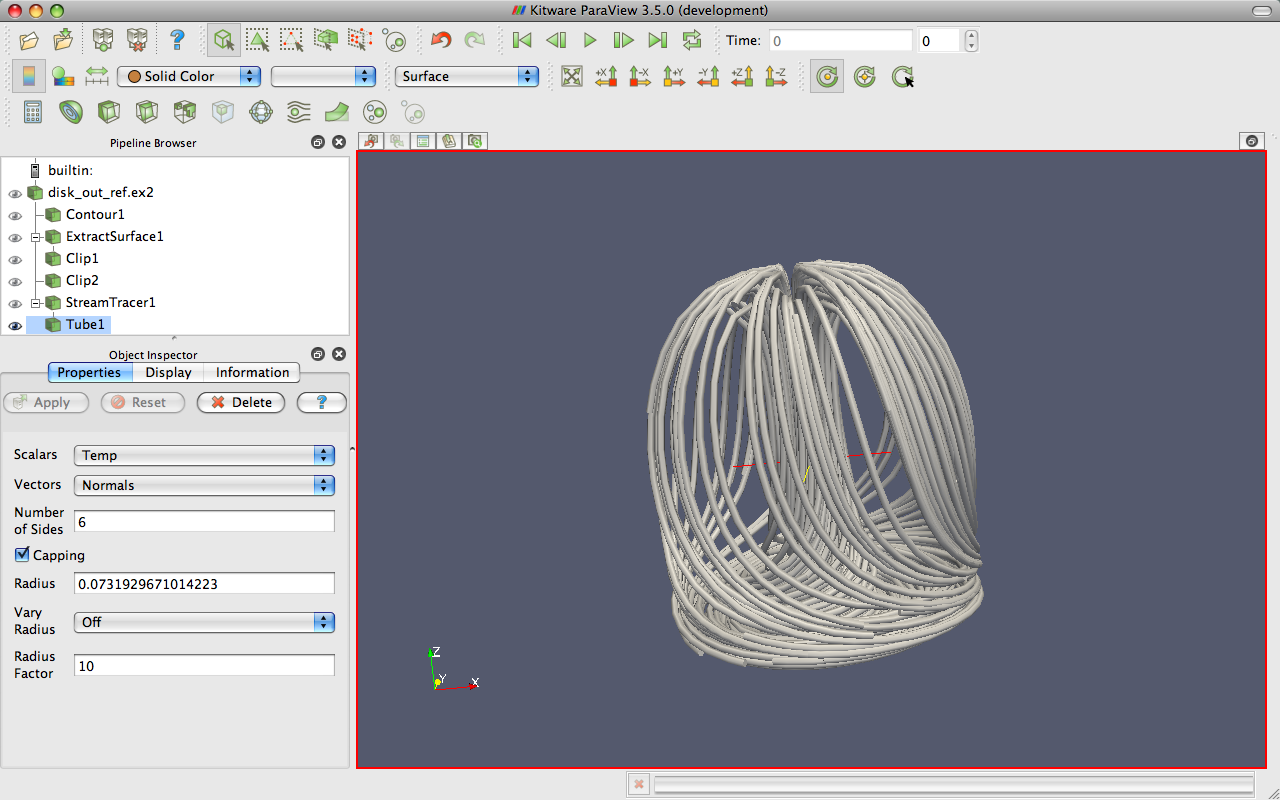
\includegraphics[width=3in]{images/StreamTracer1}
\end{inlinefig}

You can now see the streamlines much more clearly.  As you look at the
streamlines from the side, you should be able to see circular convection as
air heats, rises, cools, and falls.  If you rotate the streams to look down
the Z axis at the bottom near where the heated plate should be, you will
also see that the air is moving in a circular pattern due to the friction
of the rotating disk.

Now we can get a little fancier.  We can add glyphs to the streamlines to
show the orientation and magnitude.

\begin{enumerate}
\item Select \gui{StreamTracer1} in the pipeline browser.
\item Add the glyph filter~\glyph to \gui{StreamTracer1}.
\item In the object inspector, change the \gui{Vectors} option (second
  option from the top) to \gui{V}.
\item In the object inspector, change the \gui{Glyph Type} option (third
  option from the top) to \gui{Cone}.
\item Hit the \apply button.
\item Color the glyphs with the \gui{Temp} variable.
\end{enumerate}

\begin{inlinefig}
  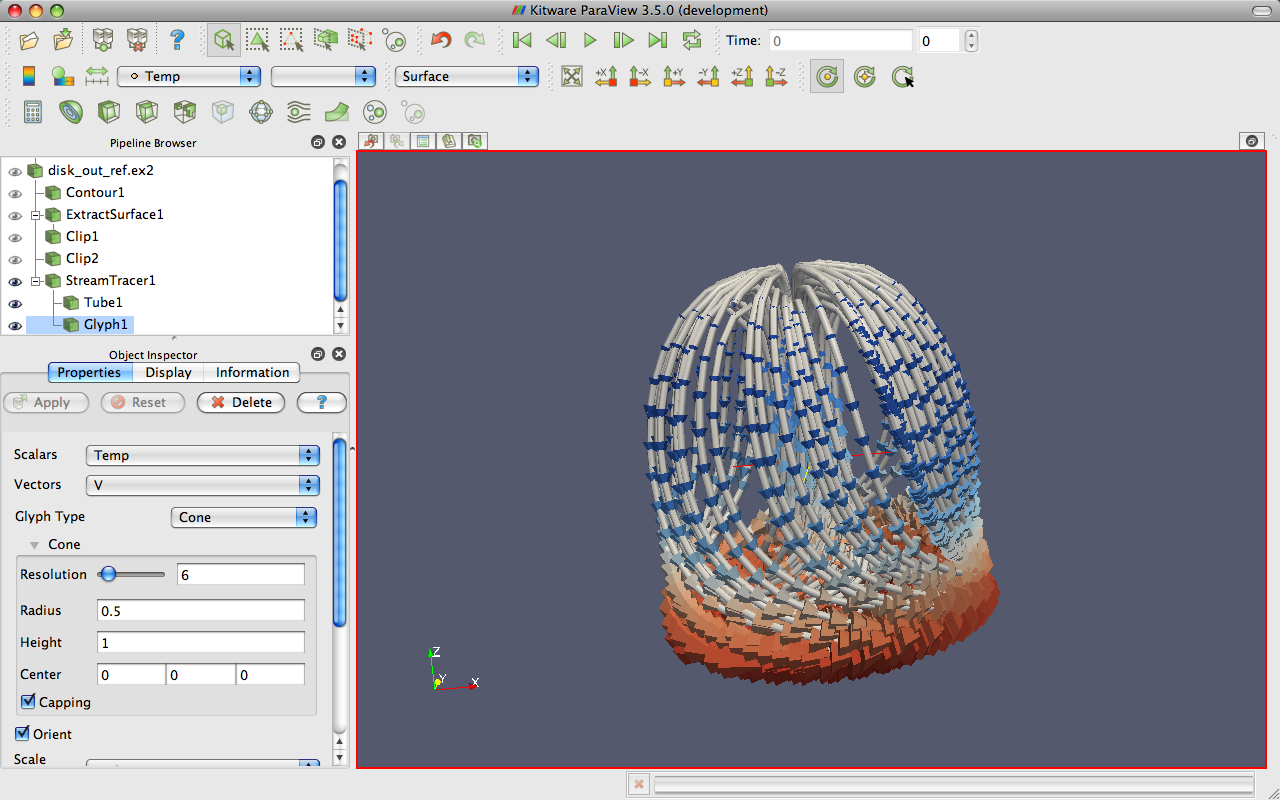
\includegraphics[width=3in]{images/StreamTracer2}
\end{inlinefig}

Now the streamlines are augmented with little pointers.  The pointers face
in the direction of the velocity, and their size is proportional to the
magnitude of the velocity.  Try using this new information to answer the
following questions.

\begin{itemize}
\item Where is the air moving the fastest?  Near the disk or away from it?
  At the center of the disk or near its edges?
\item Which way is the plate spinning?
\item At the surface of the disk, is air moving toward the center or away
  from it?
\end{itemize}

When you are done, you can restore all of your views by pressing the
restore button~\restoreView on the view toolbar.  Right click on the new
view and select \gui{Link Camera...} and then link the camera with either
of the other two views.  Now all three views have their cameras linked
together.


\section{Plotting}

ParaView's plotting capabilities provide a mechanism to drill down into
your data to allow quantitative analysis.  Plots are usually created with
filters, and all of the plotting filters can be found in the \gui{Data
  Analysis} submenu of \gui{Filters}.  Let us create a filter that will
plot the values of the mesh’s fields over a line in space.

\begin{enumerate}
\item Click on \gui{disk\_out\_ref.ex2} in the pipeline browser to make
  that the active object.
\item From the menu bar, select \gui{Filters} \ra \gui{Data Analysis} \ra
  \gui{Plot Over Line}~\icon{pqPlotLineOverTime24}. \index{plot~over~line}
  \savecounter
\end{enumerate}

\begin{inlinefig}
  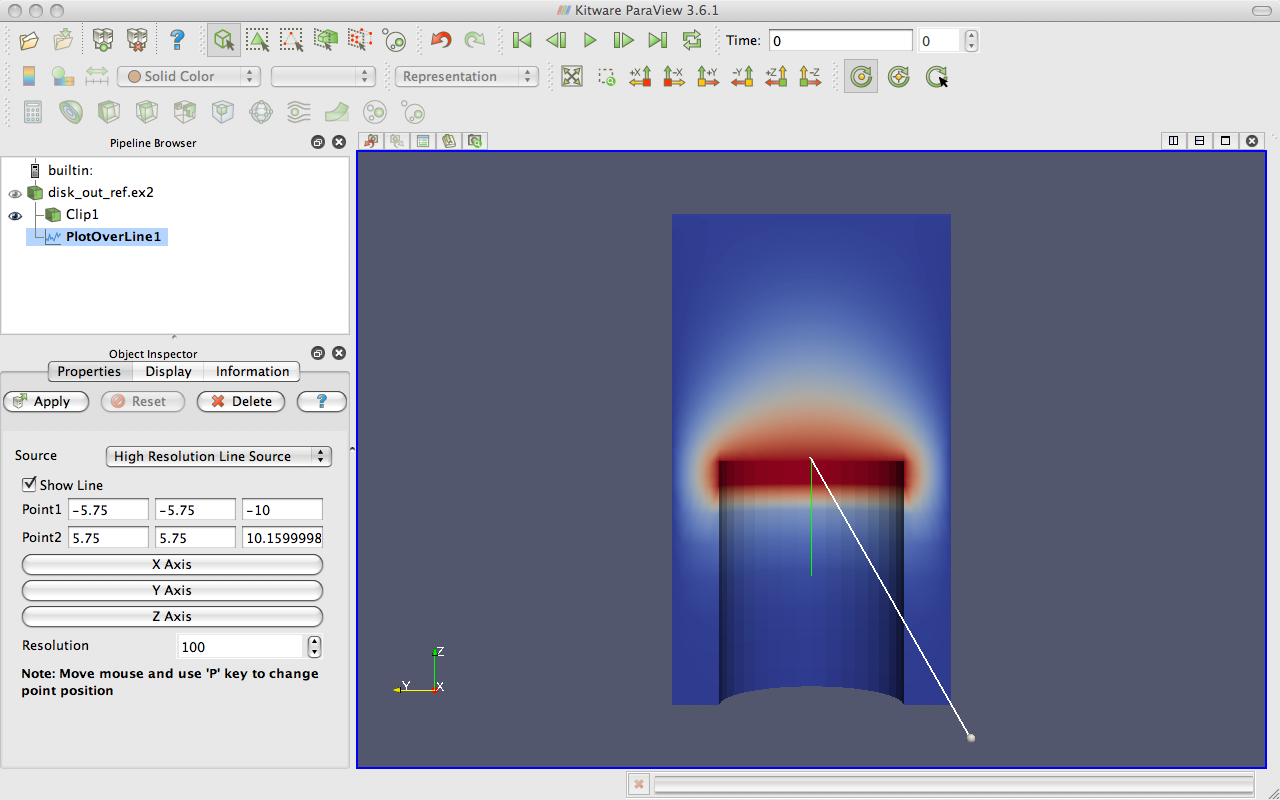
\includegraphics[width=3in]{images/LinePlot1}
\end{inlinefig}

In the active view you will see a line through your data with a ball at
each end.  If you move your mouse over either of these balls, you can drag
the balls through the 3D view to place them.  Notice that each time you
move the balls some of the fields in the object inspector also change.  You
can also place the balls by moving your mouse over the target location and
hitting the p key.  This will alternatively place each ball at the surface
underneath the mouse curser.  Note that placing the endpoints in this
manner only works when rendering solid surfaces.  It will not work with a
volume rendered image.

This representation is called a \keyterm{3D widget} because it is a GUI
component that is manipulated in 3D space.  There are many examples of 3D
widgets in ParaView.  This particular widget, the line widget, allows you
to specify a line segment in space.  Other widgets allow you to specify
points or planes.

\begin{enumerate}
  \restorecounter
\item Adjust the line so that it goes from the base of the disk straight up
  to the top of the mesh using the 3D widget manipulators, the p key
  shortcut, or the object inspector parameters.
\item Once you have your line satisfactorily located, click the \apply
  button.
\end{enumerate}

\begin{inlinefig}
  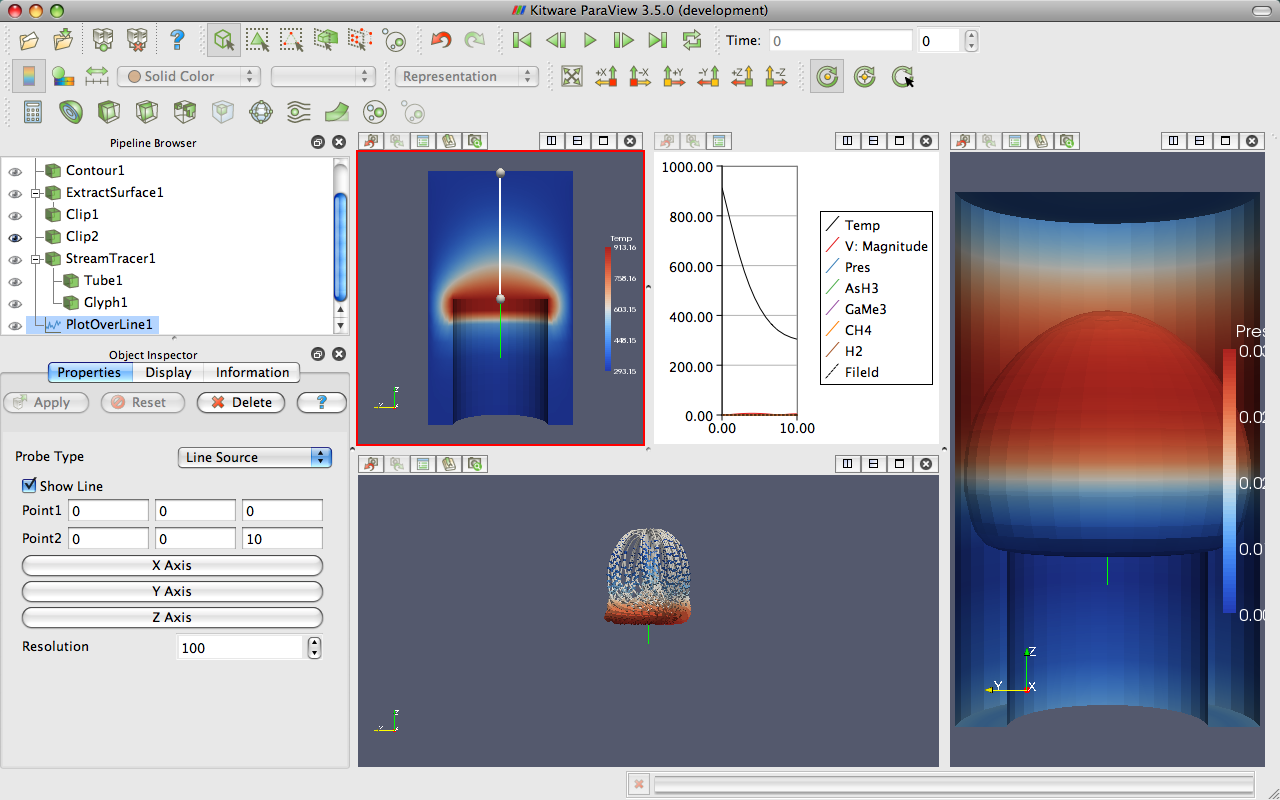
\includegraphics[width=3in]{images/LinePlot2}
\end{inlinefig}

There are several interactions you can do with the plot.  Drag with the
middle button up and down to zoom in and out.  Drag with the right button
to do a rubber band zoom.  Drag with the left button to scroll the plot
around.  You can also use the reset camera command~\resetCamera to restore
the view to the full domain and range of the plot.

Plots, like 3D renderings, are considered views.  Both provide a
representation for your data; they just do it in different ways.  Because
plots are views, you interact with them in much the same ways as with a 3D
view.  If you look in the \gui{Display} tab of the object inspector, you
will see many options on the representation for each line of the plot
including colors, line styles, vector components, and legend names.
\begin{inlinefig}
  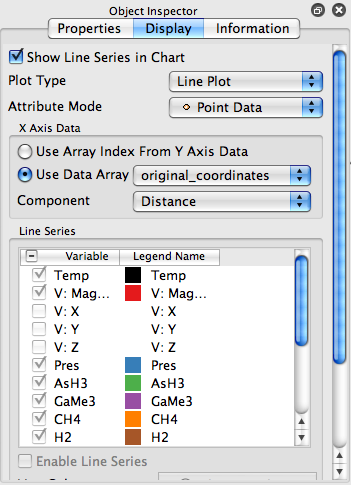
\includegraphics[width=1.5in]{images/PlotDisplayTab}
\end{inlinefig}
Plots also have a \icon{pqOptions16} button that brings up a dialog that
allows you to change plot-wide options such as labels, legends, and axes
ranges.
\begin{inlinefig}
  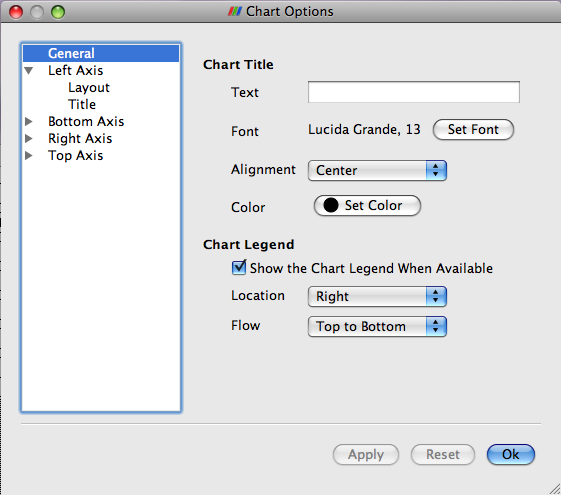
\includegraphics[width=2in]{images/PlotViewOptions}
\end{inlinefig}
Like any other views, you can capture the plot with the \gui{File} \ra
\icon{pqCaptureScreenshot24}~\gui{Save Screenshot}.  As an added bonus, you
can save can save the plot in a vector PDF format so that it scales well if
included in reports and other documents.  You can also move around plots
like you can other views.

We can use these features to get more information out of our plot.
Specifically, we can use the plot to compare the pressure and temperature
variables.

\begin{enumerate}
\item Choose a place in your GUI that you would like the plot to go and try
  using the split, delete, resize, and swap view features to move it there.
\item Make the plot view active, go to the \gui{Display} tab, and turn off
  all variables except \gui{Temp} and \gui{Pres}.
  \savecounter
\end{enumerate}

The \gui{Temp} and \gui{Pres} variables have different units.  Putting them
on the same scale is not useful.  We can still compare them in the same
plot by placing each variable on its own scale.  The line plot in ParaView
allows for a different scale on the left and right axis, and you can scale
each variable individually on each axis.

\begin{enumerate}
  \restorecounter
\item Select the \gui{Pres} variable in the \gui{Display} tab.
\item Change the \gui{Chart Axis} to \gui{Bottom - Right}
\end{enumerate}

\begin{inlinefig}
  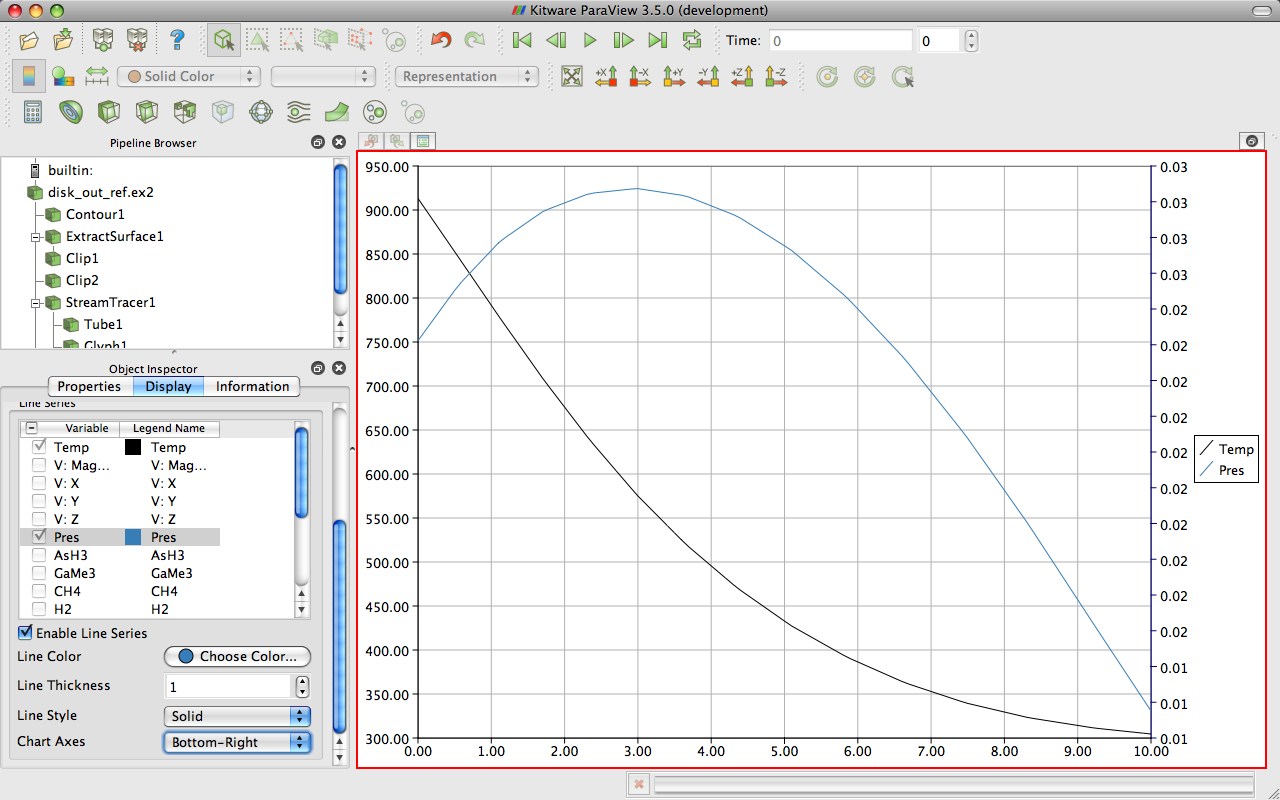
\includegraphics[width=3in]{images/LinePlot3}
\end{inlinefig}

From this plot we can verify some of the observations we made in
Section~\ref{sec:Multiview}.  We can see that the temperature is maximal at
the plate surface and falls as we move away from the plate, but the
pressure goes up and then back down.  In addition, we can observe that the
maximal pressure (and hence the location where the forces on the air are
equalized) is three units away from the disk.

The ParaView framework is designed to any number of different types of
views.  This is to provide researchers and developers a way to deliver new
ways of looking at data.  To see another example of view, select
\gui{disk\_out\_ref.ex2} in the pipeline browser, and then select
\gui{Filters} \ra \gui{Data Analysis} \ra
\gui{Histogram}~\icon{pqHistogram24}. \index{histogram} Make the histogram
for the Temp variable, and then hit the \apply button.

\begin{inlinefig}
  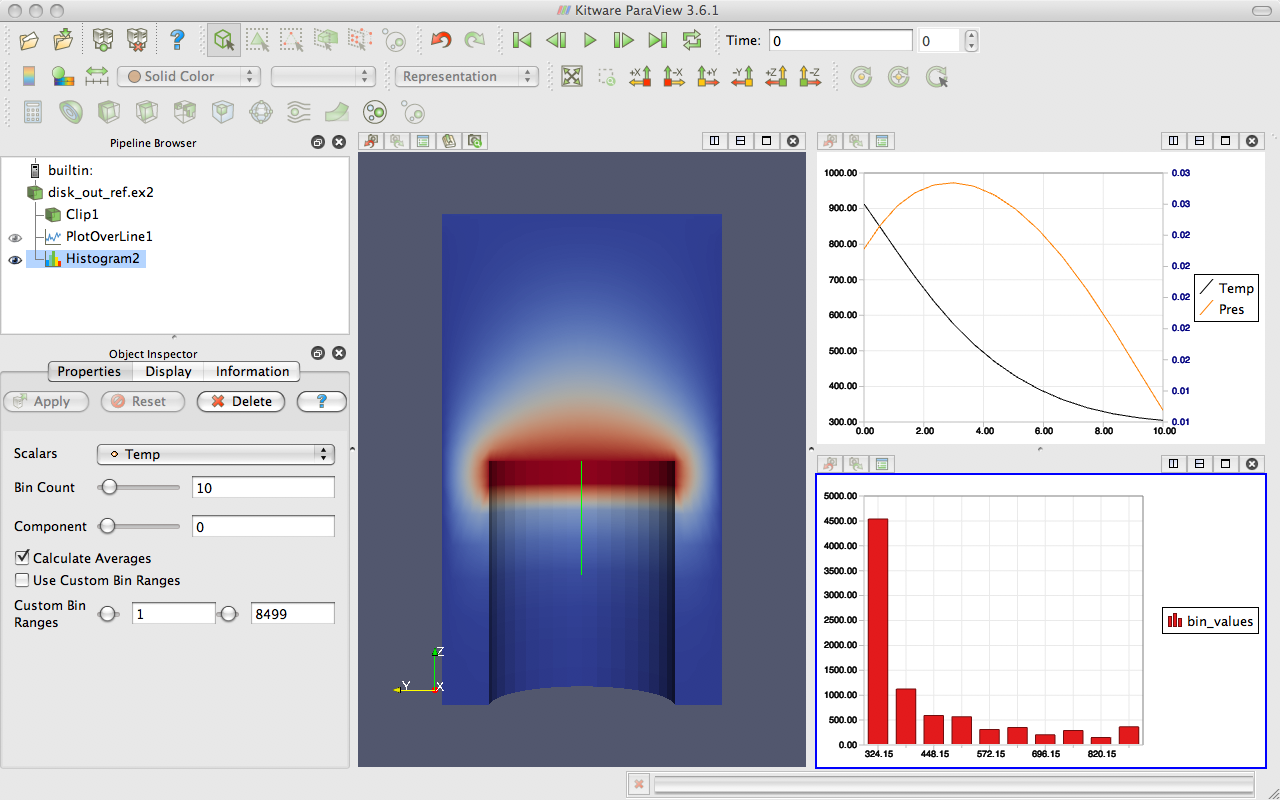
\includegraphics[width=3in]{images/HistogramPlot}
\end{inlinefig}


\section{Volume Rendering}

ParaView has several ways to represent data.  We have already seen some
examples: surfaces, wireframe, and a combination of both.  ParaView can
also render the points on the surface or simply draw a bounding box of the
data.

\begin{inlinefig}
  \begin{tabular}{c@{\;}c@{\;}c@{\;}c@{\;}c}
    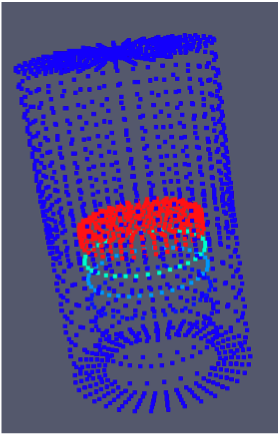
\includegraphics[width=.18\linewidth]{images/RepresentationPoints} &
    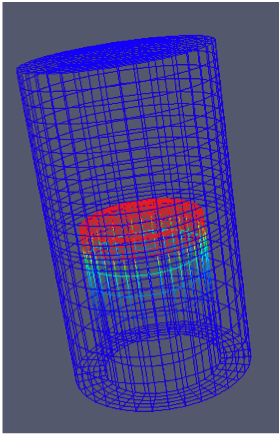
\includegraphics[width=.18\linewidth]{images/RepresentationWireframe} &
    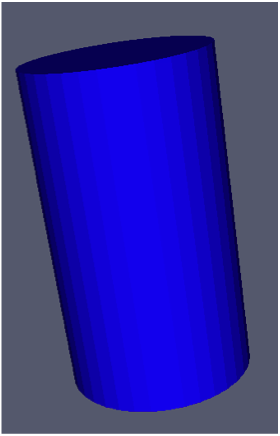
\includegraphics[width=.18\linewidth]{images/RepresentationSurface} &
    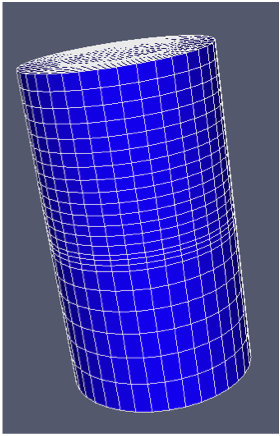
\includegraphics[width=.18\linewidth]{images/RepresentationSurfaceEdges} &
    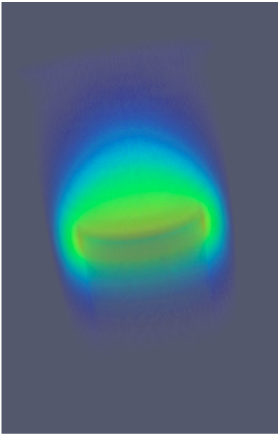
\includegraphics[width=.18\linewidth]{images/RepresentationVolume}
    \\
    Points &
    Wireframe &
    Surface &
    \parbox[t]{.18\linewidth}{\centering{}Surface with Edges} &
    Volume
  \end{tabular}
\end{inlinefig}

A powerful way that ParaView lets you represent your data is with a
technique called \keyterm{volume rendering}.  With volume rendering, a
solid mesh is rendered as a translucent cloud with the scalar field
determining the color and density at every point in the cloud.  Unlike with
surface rendering, volume rendering allows you to see features all the way
through a volume.

Volume rendering is enabled by simply changing the representation of the
object.  Let us replace the view of the temperature with a volume rendering
of the data.

\begin{enumerate}
\item Select the view showing the temperature on the surface of the clipped
  mesh.
\item Delete the clip filter that is visible.  First select the filter in
  the pipeline and then hit the \delete button.  The clipped mesh will be
  replaced with the full solid mesh (\gui{disk\_out\_ref.ex2}).
\item Make sure \gui{disk\_out\_ref.ex2} is selected in the pipeline
  browser.  Change the variable viewed to \gui{Temp} and change the
  representation to \gui{Volume}.
\end{enumerate}

\begin{inlinefig}
  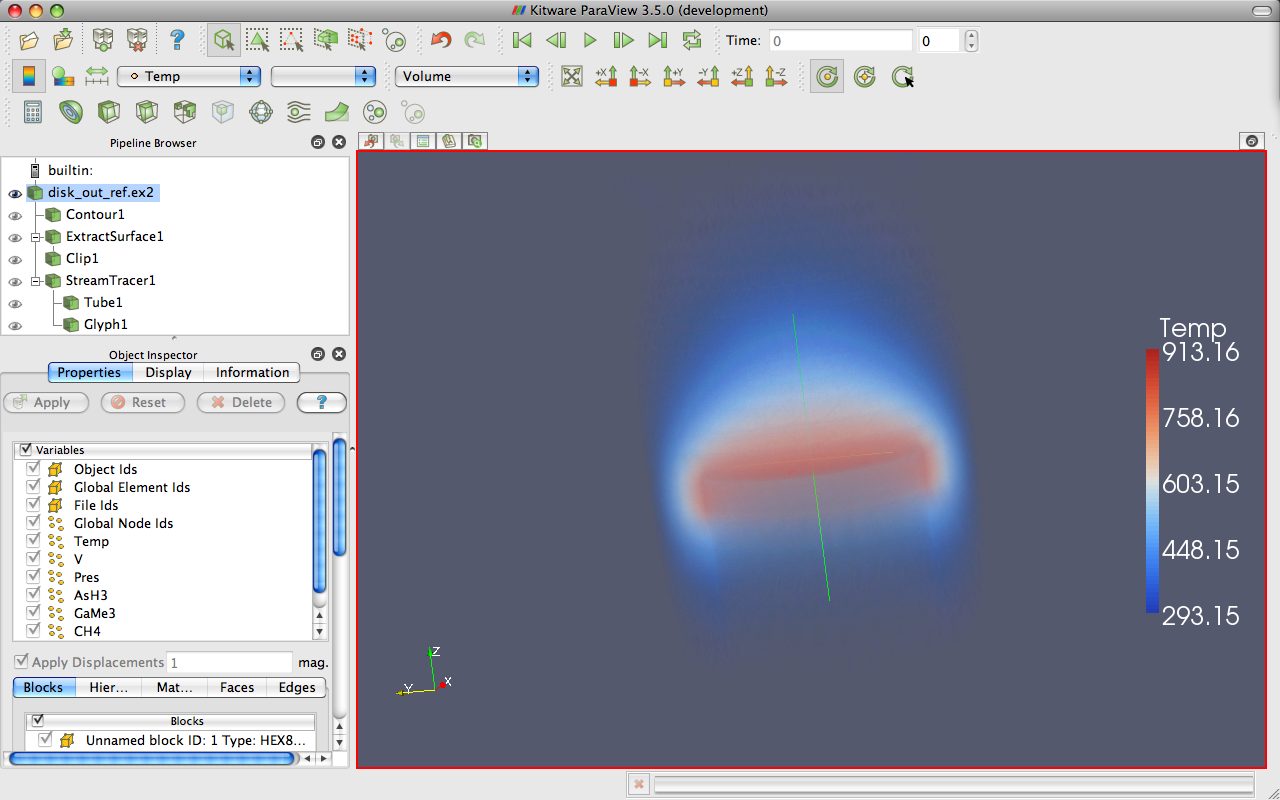
\includegraphics[width=3in]{images/VolumeRender1}
\end{inlinefig}

The solid opaque mesh is replaced with a translucent volume. You may notice
that when rotating the image is temporarily replaced with a simpler image
for performance reasons, we will discuss this feature in more detail later.
A useful feature of ParaView’s volume rendering is that it can be mixed
with the surface rendering of other objects.  This allows you to add
context to the volume rendering or to mix visualizations for a more
information-rich view.  For example, we can add a volume rendering of the
temperature to the view containing the streamlines.

\begin{enumerate}
\item Select the view showing the streamlines.
\item Click on the \eyeballg next to \gui{disk\_out\_ref.ex2} in the
  pipeline browser to make it visible and also click on the label
  \gui{disk\_out\_ref.ex2} itself to select that object.
\item Change the variable viewed to \gui{Temp} and change the
  representation to \gui{Volume}.
\end{enumerate}

\begin{inlinefig}
  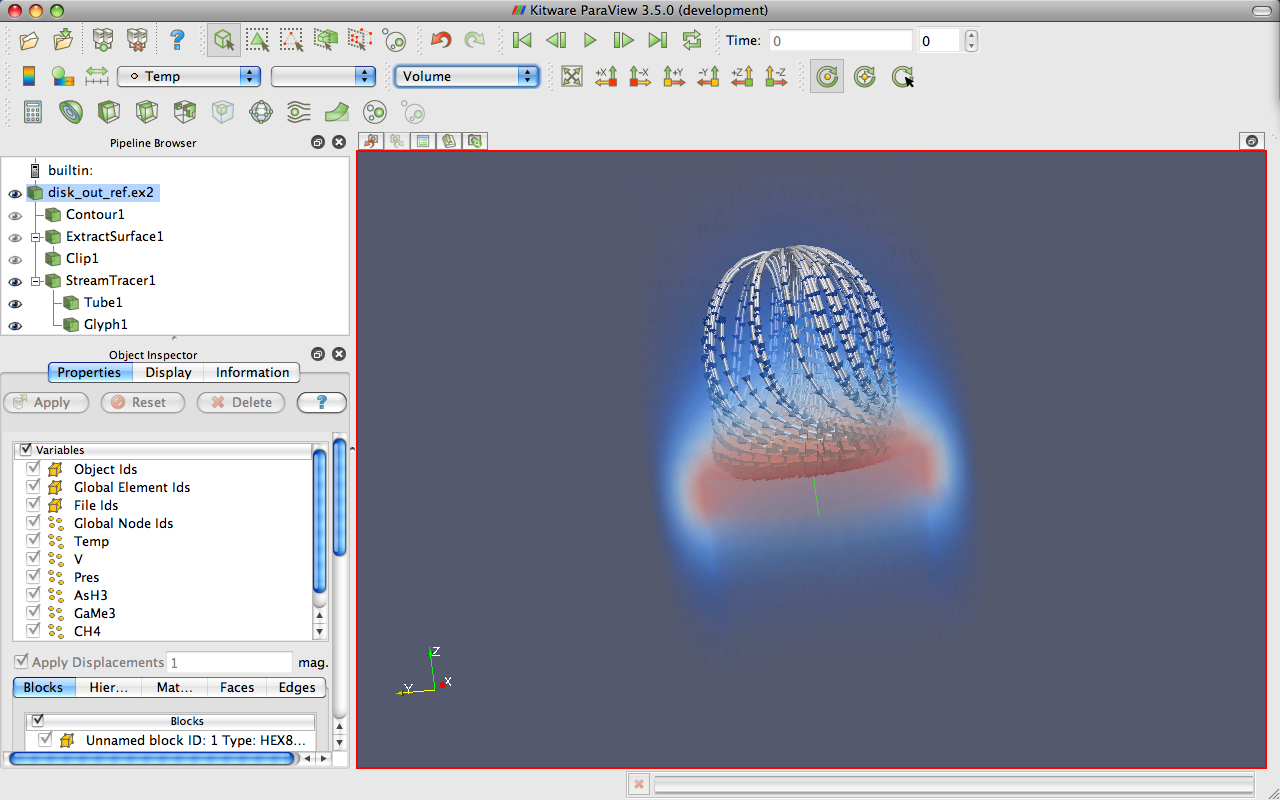
\includegraphics[width=3in]{images/VolumeRender2}
\end{inlinefig}

The streamlines are now shown in context with the temperature throughout
the volume.

By default, ParaView will render the volume with the same colors as used on
the surface with the transparency set to 0 for the low end of the range and
1 for the high end of the range.  ParaView also provides an easy way to
change the \keyterm{transfer function}, how scalar values are mapped to
color and transparency.  With the volume rendered object selected in the
pipeline browser, click on the edit color map~\icon{pqEditColor24} button.

\begin{inlinefig}
  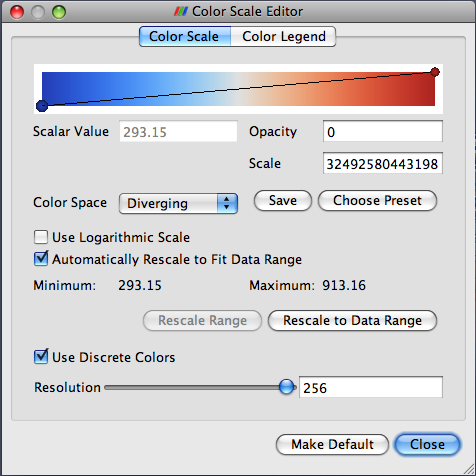
\includegraphics[width=2.5in]{images/ColorScaleEditor}
\end{inlinefig}

The resulting dialog box provides options for editing the transfer
function.  The colorful box at top displays the colors of the transfer
function with a plot of the transparency in black.  The dots on the
transfer function represent the \keyterm{control points}.  The control
points are the specific color and opacity you set at particular scalar
values, and the colors and transparency are interpolated between them.
Clicking on a blank spot in the bar will create a new control point.
Clicking on an existing control point will select it.  The selected control
point can be dragged throughout the box to change its scalar value and
transparency, and clicking again on the selected control point will bring
up a dialog box.  The selected control point will be deleted when you hit
the backspace or delete key.  Try adding and changing control points now.

Directly below the color bar are text entry widgets to numerically specify
the \gui{Scalar Value} or \gui{Opacity} of the selected control point.  The
Scale parameter adjusts the unit length of the opacity calculation.  Larger
numbers make the volume less opaque.  The \gui{Color Space} parameter
changes how colors are interpolated.  This parameter has no effect on the
color at the control points, but can drastically affect the colors between
the control points.  You can also change to a logarithmic scaling of colors
via the \gui{Use Logarithmic Scale} checkbox.

Setting up a transfer function can be tedious, so you can save it by
clicking the \includeinlinegraphics{images/ColorMapSave} button.  The
\includeinlinegraphics{images/ColorMapChoosePreset} button brings up a
dialog that allows you to manage and apply the color maps that you have
created as well as several provided by ParaView.  Press
\includeinlinegraphics{images/ColorMapChoosePreset} now, select
\gui{Black-Body Radiation} in the dialog box, and then click \gui{OK}.  Now
your volume rendering looks more representative of heat.

\begin{inlinefig}
  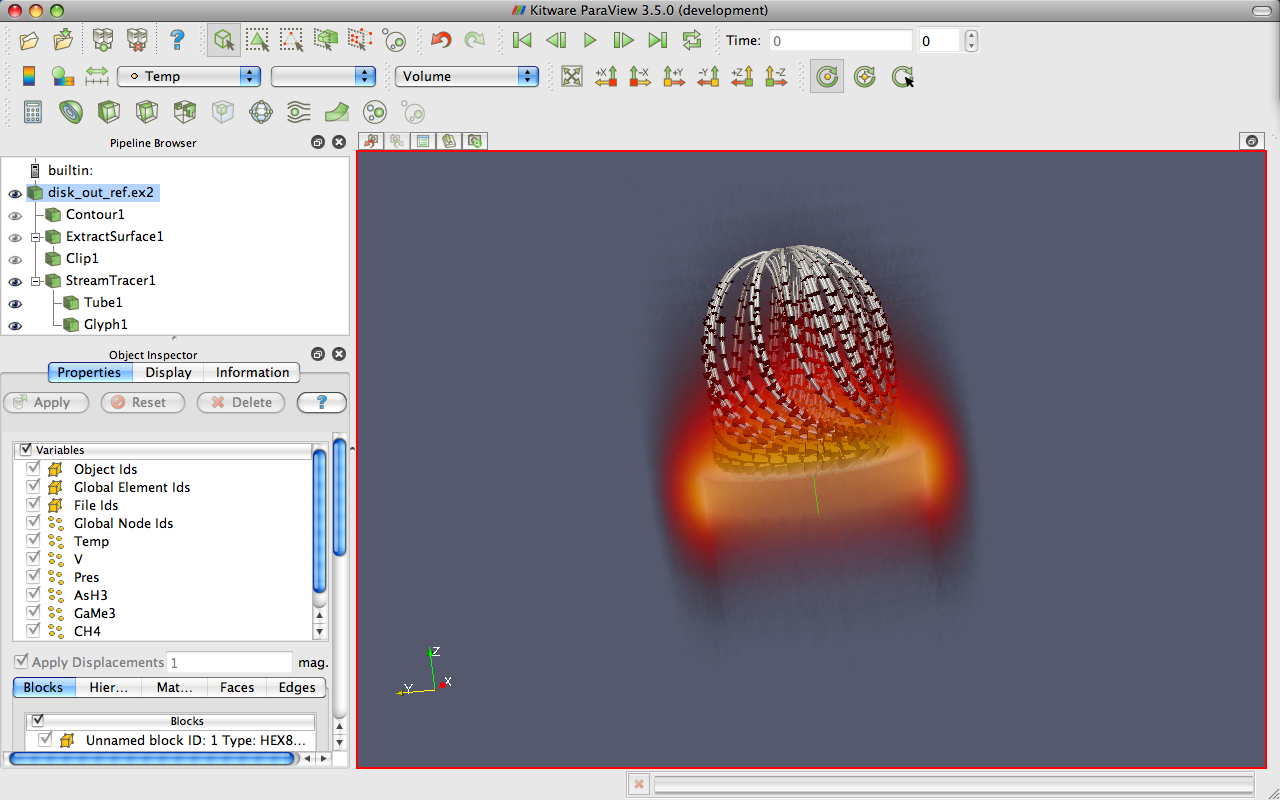
\includegraphics[width=3in]{images/VolumeRender3}
\end{inlinefig}

Notice that not only did the color mapping in the volume rendering change,
but the color mapping for \gui{Temp} in all views, including the bar chart,
changed.  This ensures consistency between the views and avoids any
confusion from mapping the same variable with different colors or different
ranges.


\section{Time}

Now that we have thoroughly analyzed the disk\_out\_ref simulation, we will
move to a new simulation to see how ParaView handles time.  First let us
clear out all of the data and start fresh.  The easiest way to do this is
to press the~\disconnect button.  We will discuss what this does later in more
detail, but for now just know that it is roughly the equivalent of
restarting ParaView.

\gui{Open} the file \gui{can.ex2}.  This is another simple simulation, this
time with data that changes over time.

\begin{inlinefig}
  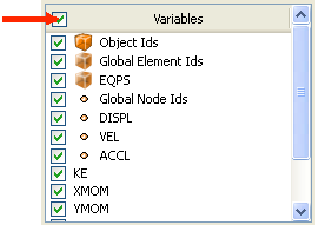
\includegraphics{images/Variables_can}
\end{inlinefig}

As before, click the checkbox in the header of the variable list to turn on
the loading of all the variables and hit the \apply button.

Press the~\yPlus button to orient the camera to the mesh.  Now press the
play button~\vcrPlay in the toolbars and watch ParaView animate the mesh to
crush the can with the falling brick.

\begin{inlinefig}
  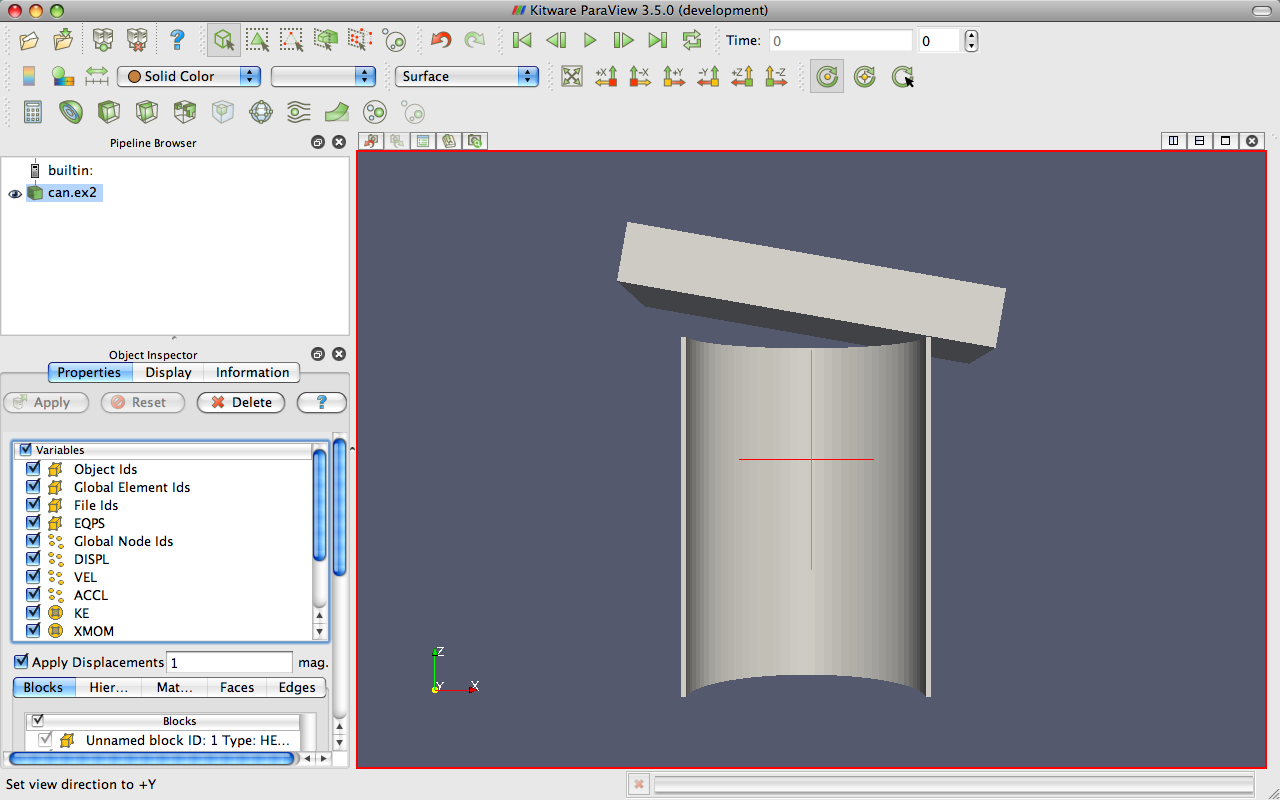
\includegraphics[width=.32\linewidth]{images/AnimateCan1}
  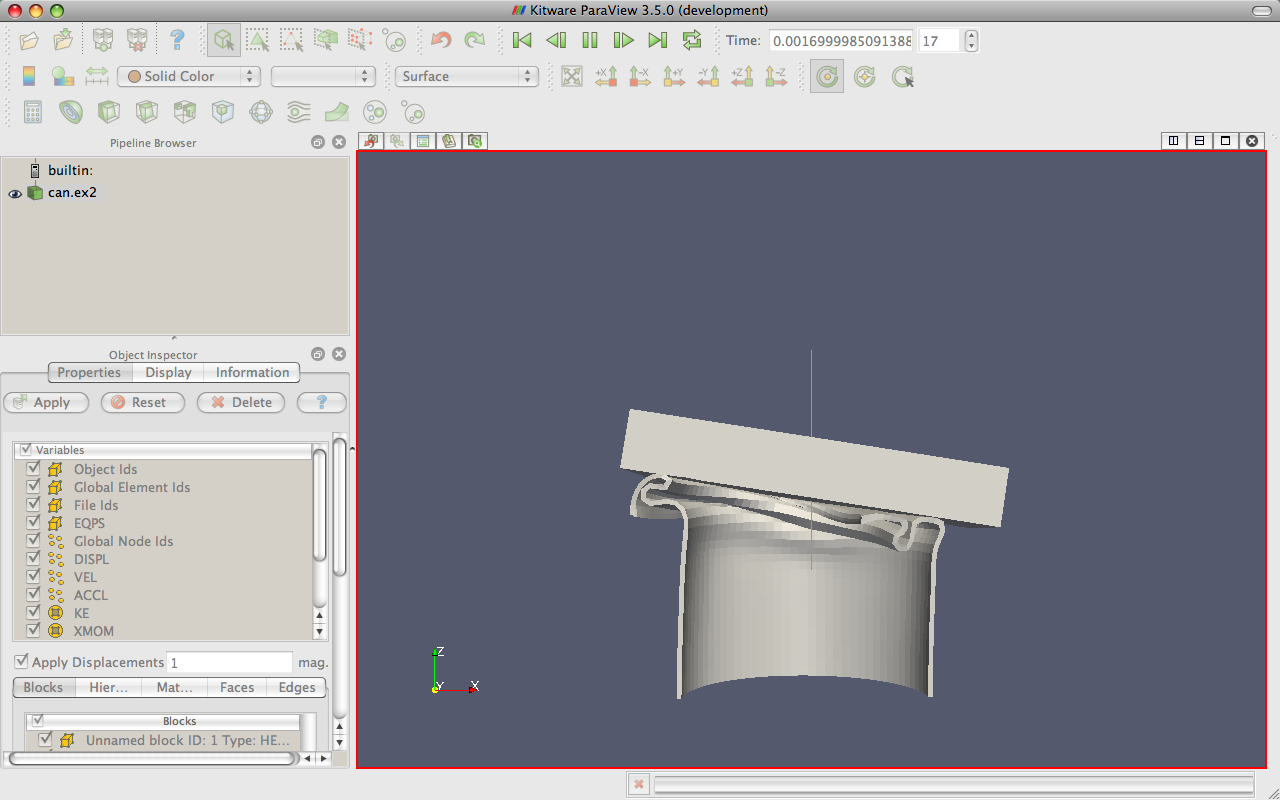
\includegraphics[width=.32\linewidth]{images/AnimateCan2}
  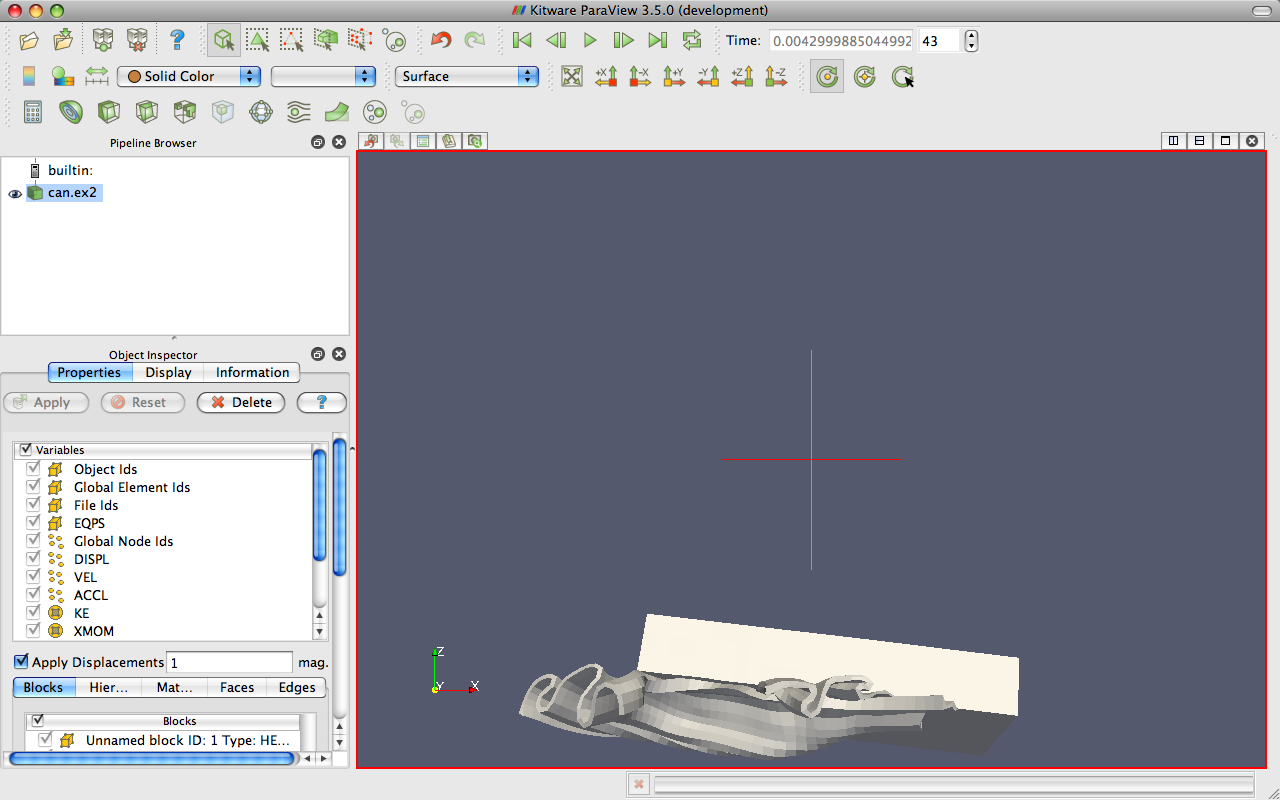
\includegraphics[width=.32\linewidth]{images/AnimateCan3}
\end{inlinefig}

That is really all there is to dealing with data that is defined over time.
ParaView has an internal concept of time and automatically links in the
time defined by your data.  Become familiar with the toolbars that can be
used to control time.

\begin{inlinefig}
  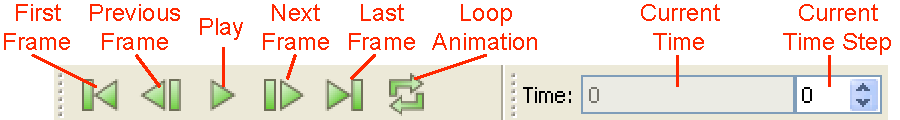
\includegraphics[width=\linewidth]{images/AnimationToolbar}
\end{inlinefig}

Saving an animation is equally as easy.  From the menu, select \gui{File}
\ra \gui{Save Animation}.  ParaView provides dialogs specifying how you
want to save the animation, and then automatically iterates and saves the
animation.

The biggest pitfall users run into is that with mapping a set of colors
whose range changes over time.  To demonstrate this, go to the first time
step~\vcrFirst, turn on the \gui{EQPS} variable, and then turn on the color
legend~\icon{pqScalarBar32}.  Now play~\vcrPlay through the animation (or
skip to the last time step~\vcrLast).  The coloring is now not very useful.
To quickly fix the problem, click the Rescale to Data
Range~\icon{pqResetRange24} button.

Although this seems like a bug, it is not.  It is the consequence of two
unavoidable behaviors.  First, when you turn on the visibility of a scalar
field, the range of the field is set to the range of values in the current
time step.  Ideally, the range would be set to the max and min over all
time steps in the data.  However, that would require ParaView to load in
all of the data on the initial read, and that would be prohibitively slow
for large data.  Second, when you animate over time, it is important to
hold the color range fixed even if the range in the data changes.  Changing
the scale of the data as an animation plays causes a misrepresentation of
the data.  It is far better to let the scalars go out of the original color
maps range than to imply that they have not.  To get around the problem,
simply go to a representative time step and hit~\icon{pqResetRange24} or
open the edit color scale dialog box~\icon{pqEditColor24} and specify a
range for the data.


\section{Selection}

A feature that greatly improved with the release of ParaView 3 and
continues to evolve is that of selection.  Selection can take place at any
time, and ParaView maintains a current selected set that is linked between
all views.  That is, if you select something in one view, that selection is
also shown in all other views that display the same object.

ParaView allows you to select points, cells, or blocks of a single data
set.  There are also multiple ways of specifying the elements to include in
the selection including id lists of multiple varieties, spatial locations,
and scalar values.  We will explore some of the combinations now.

One of the easiest ways of creating a selection is to pick elements right
inside the 3D view.  All of the 3D view selections are performed with a
\keyterm{rubber-band} selection.  That is, by clicking and dragging the
mouse in the 3D view, you will create a boxed region that will select
elements underneath it.  There are several types of rubber-band selection
that can be performed, and you initiate one by selecting one of the icons
in the selection controls toolbar or using one of the shortcut keys.  The
following 3D selections are possible.

\begin{description}
\item[\selectCellsOn Select Cells On (Surface)] Selects cells that are
  visible in the view.  (Shortcut: s)
\item[\selectPointsOn Select Points On (Surface)] Selects points that are
  visible in the view.
\item[\selectCellsThrough Select Cells Through (Frustum)] Selects all cells
  that exist under the rubber band.
\item[\selectPointsThrough Select Points Through (Frustum)] Selects all
  points that exist under the rubber band.
\item[\selectBlocks Select Blocks] Selects blocks in a
  multiblock data set.  (Shortcut: b)
\end{description}

The shortcuts s and b allow you to quickly select a cell or block,
respectively.  Use them by placing the mouse cursor somewhere in the
currently selected 3D view and hitting the appropriate key.  Then click on
the cell or block you want selected (or drag a rubber band over multiple
elements).

Experiment with the selections now.

\begin{inlinefig}
  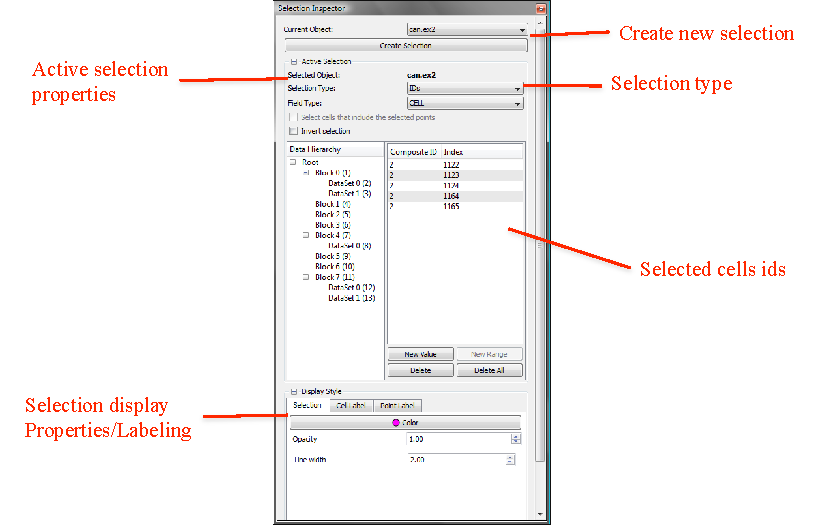
\includegraphics{images/SelectionInspector}
\end{inlinefig}

You can manage your selection with the \keyterm{selection inspector}.  You
can view the selection inspector through the menu \gui{View} \ra
\gui{Selection Inspector}.  The selection inspector allows you to view all
the points and cells in the selection as well as modify the selection.  You
can also use the selection inspector to add labels to the selection to make
it easier to identify which element is which.

Experiment with the selection inspector a bit.  Open the \gui{Selection
  Inspector}.  Then make selections using the rubber-band selection and see
the results in the \gui{Selection Inspector}.  Also experiment with
altering the selection by changing ids or inverting selections with the
\gui{Invert selection} checkbox.

You will notice that the select-on tools, \selectCellsOn/\selectPointsOn,
show a list of points/cells and the select blocks tool,~\selectBlocks,
shows a list of blocks, but the select-through tools,
\selectCellsThrough/\selectPointsThrough show neither.  That is because it
is selecting a region in space.  If you click on the \gui{Show Frustum} and
rotate the 3D view to see the region of the selection.

It should be noted that there is a fundamental difference between
selections that specify a list of points or cells and a selection that
specifies a region in space.  To understand the difference, try the
following.

\begin{enumerate}
\item Make a selection using the \gui{Select Cells
  Through}~\selectCellsThrough tool.
\item Click on the \gui{Show Frustum} checkbox in the \gui{Selection
  Inspector} and rotate the 3D view.
  \savecounter
\end{enumerate}

\begin{inlinefig}
  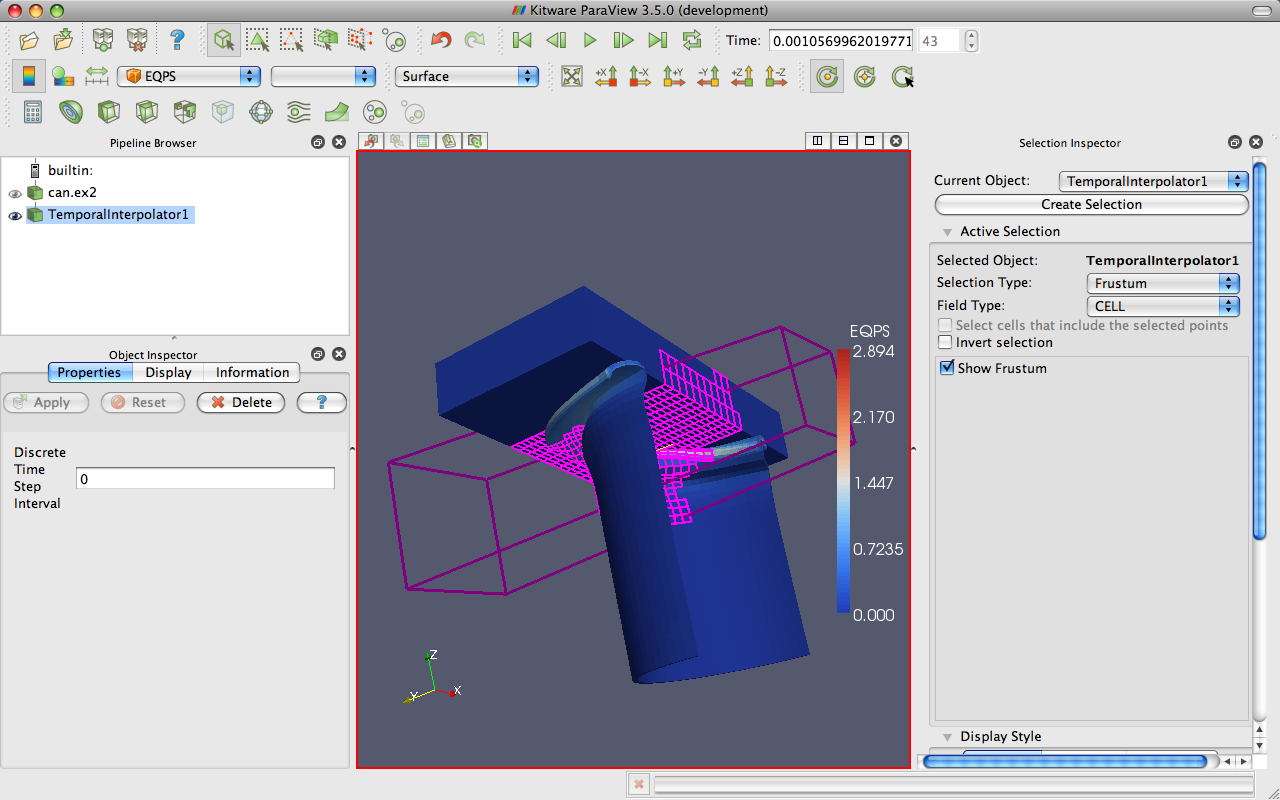
\includegraphics[width=3in]{images/SelectionFrustum}
\end{inlinefig}

\begin{enumerate}
  \restorecounter
\item Play~\vcrPlay the animation a bit.  Notice that the region remains
  fixed and the selection changes based on what cells move in or out of the
  region.
\item Change the \gui{Selection Type} to \gui{IDs}.
\item Play~\vcrPlay again.  Notice that the cells selected are fixed
  regardless of position.
\end{enumerate}

The \keyterm{spreadsheet view} is an important tool to use in combination
with selections and drill down.  The spreadsheet view allows you to read
the actual values of scalar fields and the selection mechanism will help
you identify the values of interest.

\begin{enumerate}
\item Split the view (\splitViewH or \splitViewV).
\item In the new view, click the \gui{Spreadsheet View} button.
\item Make \gui{can.ex2} visible (by clicking the appropriate \eyeballg) if
  not already visible.
  \savecounter
\end{enumerate}

As you can see, the spreadsheet view is fairly simple.  Note the two combo
boxes at the top of the spreadsheet view.  The first, \gui{Showing}, allows
you to quickly choose the data set being viewed (to avoid having to go to
the pipeline browser.  The second, \gui{Attribute}, allows you to pick
between the different types of field data.  Only one type of data
(e.g. point data or cell data) can be shown at one time because each type
results in a different number of rows and different set of columns.  The
spreadsheet view also has its own \gui{Display} panel.

\begin{inlinefig}
  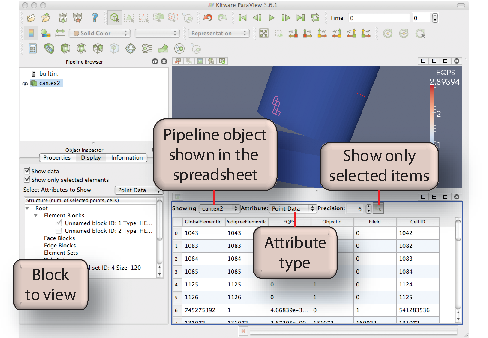
\includegraphics{images/SpreadsheetViewLabeled}
\end{inlinefig}

\begin{enumerate}
  \restorecounter
\item In the \gui{Attribute} combo box, select \gui{Cell Data}.
\item Scroll around the spreadsheet view and find some highlighted rows.
  (You may have to select a different block in the \gui{Display} panel.)
  \savecounter
\end{enumerate}

\begin{inlinefig}
  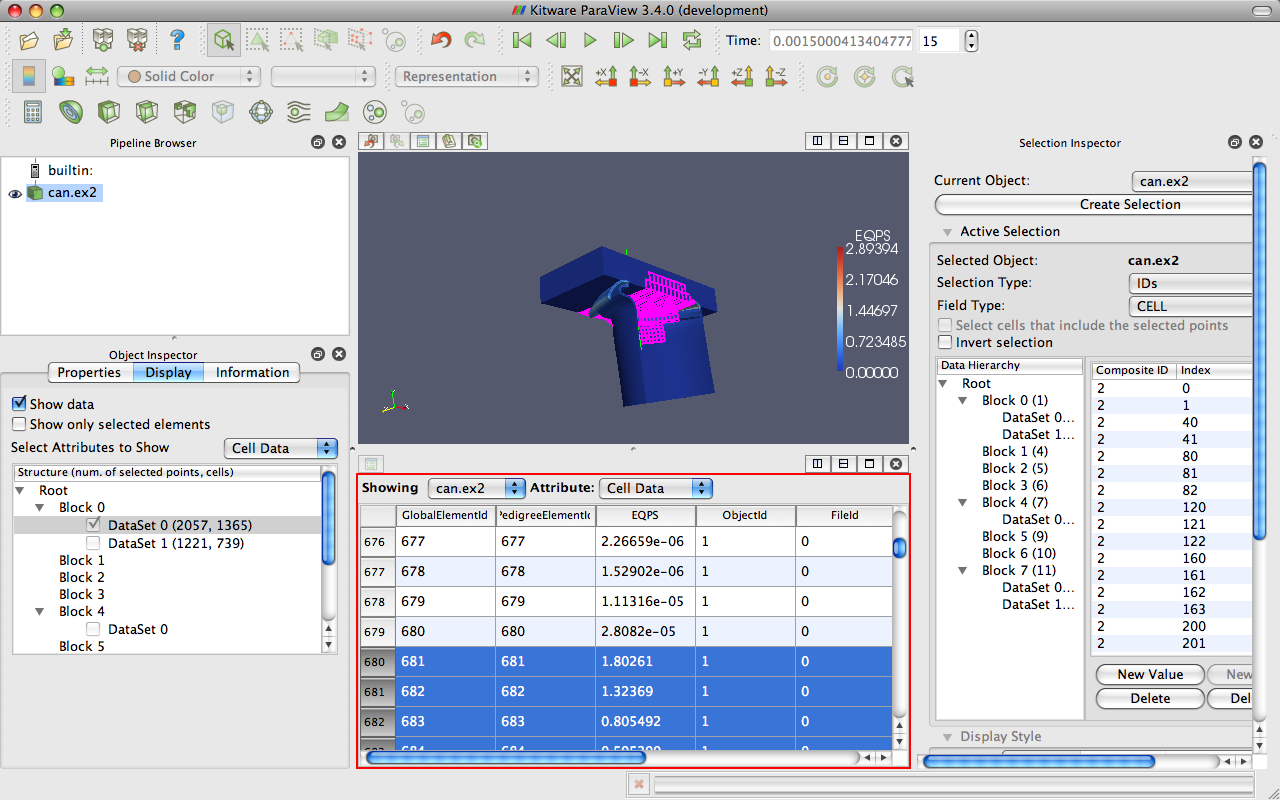
\includegraphics[width=3in]{images/SpreadsheetViewExample}
\end{inlinefig}

Those highlighted rows are the ones that are part of the current
selection.  This coordination of selection between views is an important
mechanism to link views.  In this example, it can be difficult to identify
the selected items in the spreadsheet view.  Often, you just want to see
the data in the selection.

\begin{enumerate}
  \restorecounter
\item In the \gui{Display} panel, turn on \gui{Show only selected
  elements}.
\end{enumerate}

We have now seen a selection made in the 3D view show up in the spreadsheet
view.  The linking works in reverse as well.  We can make selections in the
spreadsheet and they will be displayed in the 3D view.  In addition, we can
label the selection in the 3D view using the \gui{Selection Inspector}

\begin{enumerate}
\item Uncheck \gui{Show only selected elements}.
\item Select a few rows in the spreadsheet view.
\item Find the resulting selection in the 3D view.
\item Click the \gui{Cell Label} tab in the \gui{Selection Inspector} (at
  the bottom).
\item Check \gui{Visible}.
\item Change the \gui{Label Mode} to \gui{EQPS}.
\end{enumerate}

\begin{inlinefig}
  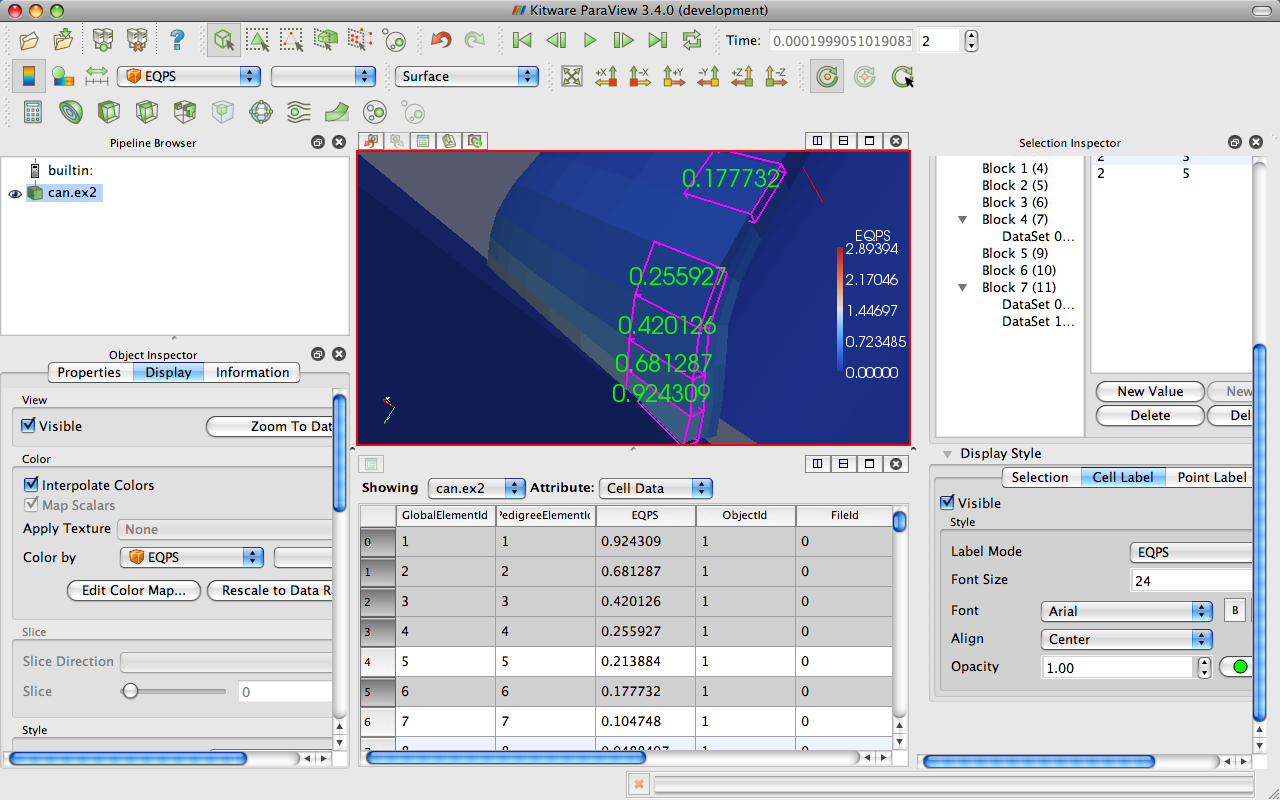
\includegraphics[width=3in]{images/SpreadsheetSelection}
\end{inlinefig}

ParaView provides the ability to plot field data over time.  Because you
seldom want to plot everything over all time, these plots work against a
selection.

\begin{enumerate}
\item With the selection still added, add the Plot Selection Over Time
  (\gui{Filters} \ra \gui{Data Analysis} \ra \gui{Plot Selection Over
  Time}~\icon{pqPlotCellOverTime24}). \index{plot~selection~over~time}
\item Click \gui{Copy Active Selection} in the \gui{Object Inspector}.
\item \apply.
\item Go to the \gui{Display} panel and select different blocks to plot
  (which correspond to each of the selected elements).
\end{enumerate}

\begin{inlinefig}
  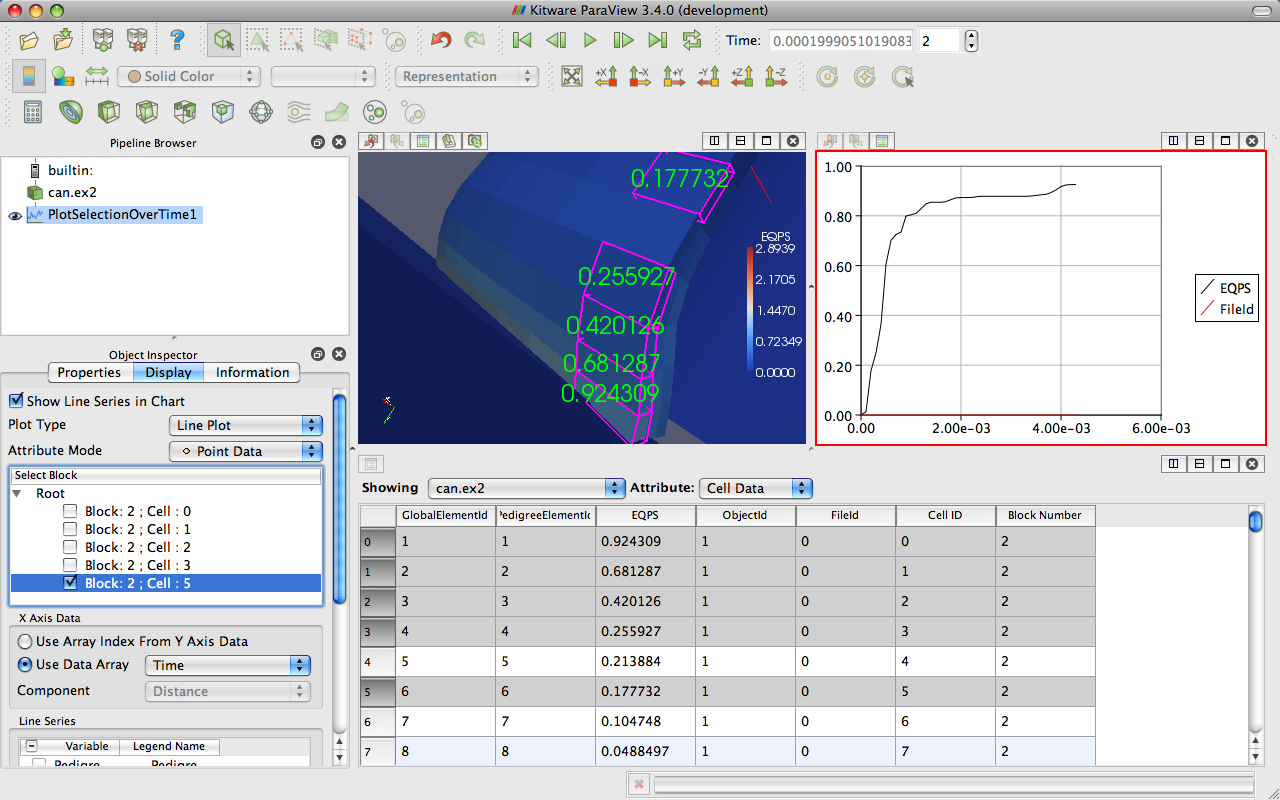
\includegraphics[width=3in]{images/PlotSelectionOverTime}
\end{inlinefig}

You can also extract a selection in order to view the selected points or
cells separately or perform some independent processing on them.  This is
done through the \gui{Extract Selection}~\icon{pqExtractSelection24}
filter.  Try this.

\begin{enumerate}
\item Turn off cell labels.
\item Make a sizable cell selection for example, with Select Cells
  Through~\selectCellsThrough.
\item Create an \gui{Extract Selection}~\icon{pqExtractSelection24} filter
  (\gui{Filters} \ra \gui{Data Analysis} \ra \gui{Extract Selection}).
  \index{extract selection}
\item Click the \gui{Copy Active Selection} button in the object inspector.
\item Hit the \apply button.
\end{enumerate}

\begin{inlinefig}
  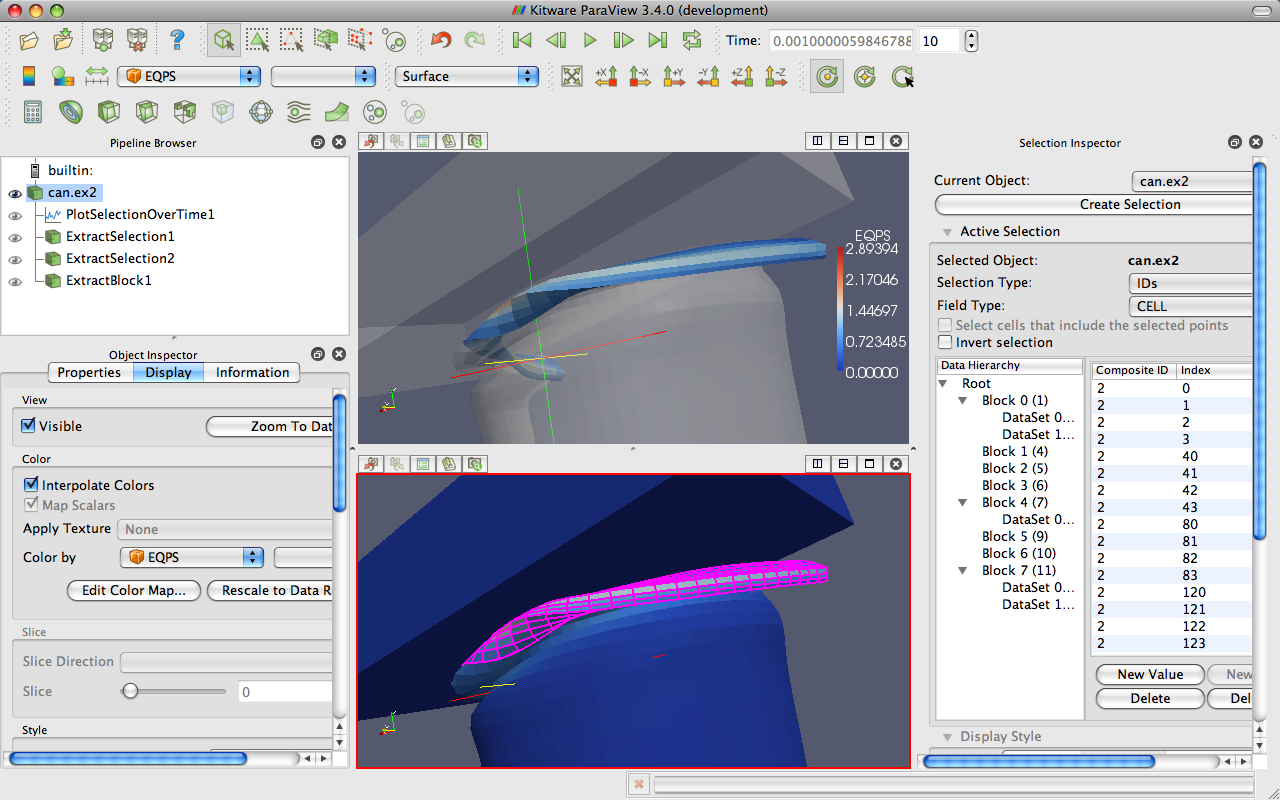
\includegraphics[width=3in]{images/ExtractSelection}
\end{inlinefig}

The object in the view is replaced with the cells that you just
selected. (Note that in this image I added a translucent surface and a
second view with the original selection to show the extracted cells in
relation to the full data.) You can perform computations on the
extracted cells by simply adding filters to the extract selection pipeline
object.

We are done with the extracted cells, so delete them (i.e. \delete the
\gui{ExtractSelection1} filter).  You can also close the \gui{Selection
  Inspector} and delete the plot and spreadsheet views; we are done with
them.  You can also \delete the \gui{PlotSelectionOverTime1} filter.


\section{Controlling Time}

% Originally this was in the Time section, but I had to move it due to a
% strange bug with the spreadsheet view and the temporal interpolator (bug
% 7701).  If that gets fixe, this section should probably go back up into
% the Time section (or at least before Selection).  Might also consider
% moving annotation before Selection so that you don't have to do that
% weird delete everything but can.

ParaView has many powerful options for controlling time and animation.  The
majority of these are accessed through the \keyterm{animation view}.  From
the menu, click on \gui{View} \ra \gui{Animation View}.

\begin{inlinefig}
  \includegraphics[width=3in]{images/AnimationView}
\end{inlinefig}

For now we will examine the controls at the top of the animation view.  The
animation \keyterm{mode} parameter determines how ParaView will step
through time during playback.  There are three modes available.

\begin{description}
\item[Sequence] Given a start and end time, break the animation into a
  specified number of frames spaced equally apart.
\item[Real Time] ParaView will play back the animation such that it lasts
  the specified number of seconds.  The actual number of frames created
  depends on the update time between frames.
\item[Snap To TimeSteps] ParaView will play back exactly those time steps
  that are defined by your data.
\end{description}

Whenever you load a file that contains time, ParaView will automatically
change the animation mode to \gui{Snap To TimeSteps}.  Thus, by default you
can load in your data, hit play~\vcrPlay, and see each time step as defined
in your data.  This is by far the most common use case.

A counter use case can occur when a simulation writes data at variable time
intervals.  Perhaps you would like the animation to play back relative to
the simulation time rather than the time index.  No problem.  We can switch
to one of the other two animation modes.  Another use case is the desire to
change the playback rate.  Perhaps you would like to speed up or slow down
the animation.  The other two animation modes allow us to do that.

Try it now.  Change the animation mode to \gui{Real Time}.  By default the
animation is set up with the time range specified by the data and a
duration of 10 seconds.  Play~\vcrPlay the animation now.  The result looks
similar, but the animation is now a linear scaling of the simulation time
and will complete in 10 seconds.

Now try changing the \gui{Duration} to 60 seconds.  The animation is
clearly playing back more slowly.  Unless your computer is updating slowly,
you will also notice that the animation is jerkier than before.  This is
because we have exceeded the temporal resolution of the data set.  Often
this is the desired behavior; it is showing you exactly what is present in
the data.  However, if you wanted to make an animation for a presentation,
you may want a smoother animation.

There is a special filter in ParaView to make this possible.  It is called
the \keyterm{temporal interpolator}.  This filter will interpolate the
positional and field data in between the time steps defined in the original
data set.  This functionality is made possible by recent advances in the
ParaView and VTK pipeline structure.  Try the filter now.  With
\gui{can.ex2} highlighted in the pipeline browser, select \gui{Filters} \ra
\gui{Temporal} \ra \gui{Temporal Interpolator}.  Hit \apply and change back
to Real Time mode in the animation view if necessary.  Also split the
view~\splitViewH, show the \gui{TemporalInterpolator1} in one, show
\gui{can.ex2} in the other, and link the cameras.  Play~\vcrPlay the
animation to see the effect.


\section{Text Annotation}

When using ParaView as a communication tool it is often helpful to annotate
the images you create with text.  With ParaView 3 it is very easy to create
text annotation wherever you want in a 3D view.  There is a special
\keyterm{text source} that simply places some text in the view.  Try it
now.

\begin{enumerate}
\item From the menu bar, select \gui{Sources} \ra \gui{Text}.
\item In the text edit box of the object inspector, type a message.
\item Hit the \apply button.
\end{enumerate}

\begin{inlinefig}
  \includegraphics[width=3in]{images/TextSource}
\end{inlinefig}

The text you entered appears in the 3D view.  You can place this text
wherever you want by simply dragging it with the mouse.  The \gui{Display}
tab in the object inspector provides additional options for the size, font,
and color of the text.  It also has additional controls for placing the
text in the most common locations.

\begin{inlinefig}
  \includegraphics[width=2in]{images/TextPosition}
\end{inlinefig}

Often times you will need to put the current time value into the text
annotation.  Typing the correct time value can be tedious an error prone
with the standard text source and impossible when making an animation.
Therefore, there is a special \keyterm{annotate time} source that will
insert the current animation time into the string.

\begin{enumerate}
\item Add an \gui{Animate Time} source (\gui{Sources} \ra \gui{Annotate
  Time}).
\item Move annotation around as necessary.
\item Play~\vcrPlay and observer how the time annotation changes.
  \savecounter
\end{enumerate}

\begin{inlinefig}
  \includegraphics[width=3in]{images/AnnotateTimeSource}
\end{inlinefig}

There are instances when the current animation time is not the same as the
time step read from a data file.  Often it is important to know what the
time stored in the data file is, and there is a special version of annotate
time that acts as a filter.

\begin{enumerate}
  \restorecounter
\item Select \gui{can.ex2}.
\item \gui{Filters} \ra \gui{Alphabetical} \ra \gui{Annotate
  Time}. \index{annotate time}
\item \apply.
\item Move annotation around as necessary.
\item Play~\vcrPlay and observer how the time annotation changes.
\end{enumerate}

\begin{inlinefig}
  \includegraphics[width=3in]{images/AnnotateTimeFilter}
\end{inlinefig}


\section{Animations}

We have already seen how to animate a data set with time in it
(hit~\vcrPlay).  However, ParaView’s animation capabilities go far beyond
that.  With ParaView you can animate nearly any property of any pipeline
object.  We will demonstrate that now, but first press the \disconnect
button to clear out the current ParaView state.  Now we are ready to make a
simple animation.

\begin{enumerate}
\item Create a sphere source (\gui{Sources} \ra \gui{Sphere}) and \apply it.
\item Now make sure the animation view panel is visible (\gui{View} \ra
  \gui{Animation View} if it is not).
\item Change the \gui{No. Frames} option to 50 (10 will go far too quickly).
\item Find the property selection widgets at the bottom of the animation
  view and select \gui{Sphere1} in the first box and \gui{Start Theta} in
  the second box.
  \begin{inlinefig}
    \includegraphics[height=1.5\baselineskip]{images/AddStartThetaTrack}
  \end{inlinefig}
  Hit the \icon{pqPlus16} button.
  \savecounter
\end{enumerate}

\begin{inlinefig}
  \includegraphics[width=4in]{images/BuildAnimation1}
\end{inlinefig}

What you have done is created a \keyterm{track} for the \gui{Start Theta}
property of the \gui{Sphere1} object.  A track is represented as horizontal
bars in the animation view.  They hold \keyterm{key frames} that specify
values for the property a specific time instance.  The value for the
property is interpolated between the key frames.  When you created a track
two key frames were created automatically: a key frame at the start time
with the minimal value and a key frame at the end time with the maximal
value.  The property you set here defines the start range of the sphere.
If you play~\vcrPlay the animation, you will see the sphere open up then
eventually wrap around itself and disappear.

\begin{inlinefig}
  \includegraphics[width=1in]{images/AnimateSphere0}
  \includegraphics[width=1in]{images/AnimateSphere1}
  \includegraphics[width=1in]{images/AnimateSphere2}
  \includegraphics[width=1in]{images/AnimateSphere3}
\end{inlinefig}

You can modify a track by double clicking on it.  That will bring up a
dialog box that you can use to add, delete, and modify key frames.

\begin{inlinefig}
  \includegraphics[width=3in]{images/AnimationKeyframesDialog}
\end{inlinefig}

Use this feature to create a new key frame in the animation.

\begin{enumerate}
  \restorecounter
\item Double-click on the \gui{Sphere1 -- Start Theta} track.
\item In the \gui{Animation Keyframes} dialog, click the \gui{New} button.
  This will create a new key frame at time 0.5.
\item Modify the first key frame value to be 360 and the second key frame
  value to be 0.
\item Click \gui{OK}.
\end{enumerate}

\begin{inlinefig}
  \includegraphics[width=4in]{images/BuildAnimation2}
\end{inlinefig}

When you play the animation, the sphere will first get bigger and then get
smaller again.

You are not limited to animating just one property.  You can animate any
number of properties you wish.  Now we will create an animation that
depends on modifying two properties.

\begin{enumerate}
\item Double-click on the \gui{Sphere1 -- Start Theta} track.
\item In the \gui{Animation Keyframes} dialog, \gui{Delete} the first track
  (at time step 0).
\item Click \gui{OK}.
\item In the animation view, create a track for the \gui{Sphere1} object,
  \gui{End Theta} property.
\item Double-click on the \gui{Sphere1 -- End Theta} track.
\item Change the time for the second key frame to be 0.5.
\end{enumerate}

\begin{inlinefig}
  \includegraphics[width=4in]{images/BuildAnimation3}
\end{inlinefig}

The animation will show the sphere creating and destroying itself, but this
time the range front rotates in the same direction.  It makes for a very
satisfying animation when you loop~\vcrLoop the animation.


\section{Scripting}

There are many ways to modify and automate ParaView.  One of the most
convenient ways to do so is to use the Python scripting that is built into
ParaView.  Although the Python bindings are beyond the scope of this
tutorial, we discuss the ways in which you can use them.  You can get more
information about the Python bindings from the ParaView Wiki
(\href{http://www.paraview.org/Wiki/images/2/26/Servermanager.pdf}{http://www.paraview.org/Wiki/images/2/26/Servermanager.pdf}).

The most straightforward way to bring up Python in ParaView is to bring up
the embedded Python shell.  In the menu, select \gui{Tools} \ra \gui{Python
  Shell}.  This brings up a dialog box with a Python shell that you can use
to issue arbitrary commands like run previously written scripts, load a
saved state, manipulate pipeline objects, and load plugins.

\begin{inlinefig}
  \includegraphics[width=2.5in]{images/PythonShell}
\end{inlinefig}

There is also a mechanism to use Python to manipulate data from within the
pipeline.  There is a special filter called the \keyterm{programmable
  filter} (accessible from \gui{Filters} \ra \gui{Data Analysis} \ra
\gui{Programmable Filter}).  This filter allows you to define a Python
script in the object inspector.  This script will be executed every time
the pipeline is updated.  The scripts have direct access to your data and
allow you to manipulate them in any way you like.  The truly great thing
about the programmable filter is that it even works in parallel mode.  If
the data is on a distributed parallel machine, the Python script is also
distributed on the machine and executes on the data in the same way it
would as if it was running in serial.  Thus, you can have parallel
scripting of your data with no further effort on your part.

Sometimes it is convenient to automate your post-processing and
visualization with a Python script that completely bypasses the ParaView
GUI (and therefore any need for user intervention).  You can do this with
the \texttt{pvpython} application that comes with ParaView.  The
\texttt{pvpython} application is simply a Python interpreter with all of
the ParaView bindings already loaded into it.  You can execute that program
with a script to completely automate ParaView.  ParaView also comes with a
similar program called \texttt{pvbatch}.  Unlike \texttt{pvpython},
\texttt{pvbatch} can run in parallel without having to establish a
client/server connection, but some of the GUI library will be unavailable.


% Chapter Basic Usage
